\documentclass[a4paper,12pt]{article} % Specify A4 paper size and font size
\usepackage{amsmath}
\usepackage{amssymb} % Include this package for \mathbb
\usepackage[margin=1in]{geometry} % Adjust the margin as needed
\usepackage{graphicx} % Include this package for \includegraphics

\begin{document}

\author{kipngeno koech - bkoech}
\title{Homework 6 - Applied Stochastic Processes}
\date{\today}
\maketitle

\medskip
\section{INTRODUCTION}
This document contains solutions to homework 6 of the course Applied Stochastic Processes. This homework focuses on exploring noisy data and denoising tecniques. Noisy data means data that is corrupted by random errors. The errors can be due to various reasons such as measurement errors, environmental factors, or even human errors. The goal of denoising is to remove the noise from the data and recover the original signal. 
\newline\newline
This homework explores the use of vairous denoising techniques such as the simple moving average, gaussian kernel \& gaussian weighted moving average, low pass butterworth filter and exponential moving average. Let us briefly discuss each of these techniques.
\newline\newline
\textbf{Simple Moving Average:} This technique involves taking the average of a fixed number of data points (a window size). The average is then used as the denoised value for the data point at the center of the window. The window size is a parameter that can be adjusted to control the amount of smoothing. You iterate through the data points and apply the moving average to each data point. The new values of your denoised data will be these averages over the windows. The larger the window size the more smoothing you will get because you are averaging over more data points.
\newline\newline
\textbf{Gaussian Kernel \& Gaussian Weighted Moving Average:} This technique involves using a Gaussian kernel to weight the data points. The Gaussian kernel is a bell-shaped curve that assigns weights to the data points. The weights are higher for the data points that are closer to the center of the kernel and lower for the data points that are further away. The weighted average is then used as the denoised value for the data point at the center of the kernel. The standard deviation of the Gaussian kernel is a parameter that can be adjusted to control the amount of smoothing. The larger the standard deviation the more smoothing you will get because you are assigning higher weights to more data points.
\newline\newline
\textbf{low pass butterworth filter:} it is a filter used to pass low-frequency components while attenuating high-frequency noise. It is a type of signal processing filter that is used to remove noise from a signal. The cutoff frequency is a parameter that can be adjusted to control the amount of smoothing. The larger the cutoff frequency the more smoothing you will get because you are removing more high-frequency noise. The order of the filter is another parameter that can be adjusted to control the amount of smoothing. The higher the order of the filter the more smoothing you will get because you are removing more high-frequency noise. 
\newline\newline
\textbf{exponential moving panel:} it assigns weights to more recent data points making it more responsive to recent changes in the data. The weights are assigned exponentially with the most recent data points having the highest weights. The smoothing parameter is a parameter that can be adjusted to control the amount of smoothing. The larger the smoothing parameter the more smoothing you will get because you are assigning higher weights to more recent data points.
\section{ANALYSIS}
\subsection{Quality Control with Noisy Measurements}
\textbf{problem: }A factory produces light bulbs, and each has a 60\% probability of passing
quality control. However, noise in the measurements causes some pass/fail outcomes to
be flipped.
\subsubsection{ Denoising with Simple Moving Average}
with a window size of 10, the simple moving average denoising technique was applied to the data. The results are shown in figure 1. The denoised data is shown in red while the original data is shown in dashed green. The True mean of the data is \(\textbf{0.61}\) while the denoised mean is \(\textbf{0.58}\) and Noisy mean is \(\textbf{0.58}\)
\begin{figure}[h]
\centering
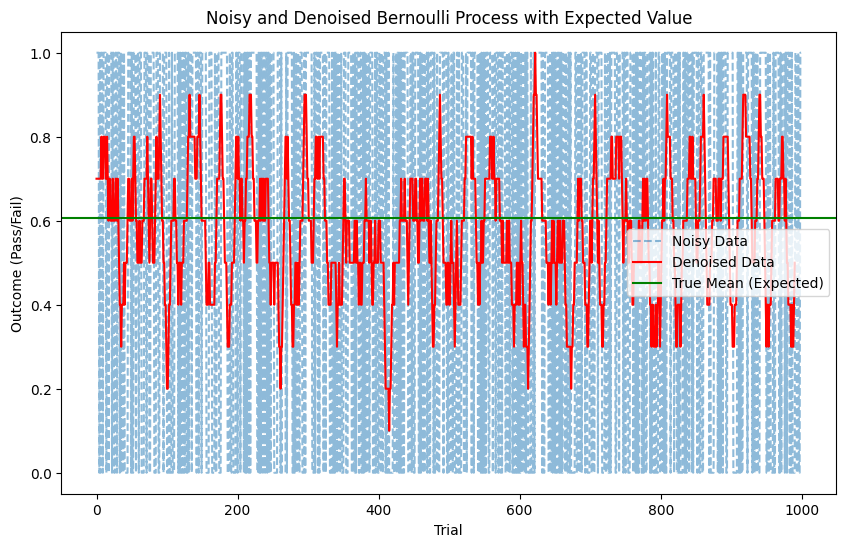
\includegraphics[width=0.8\textwidth]{simple_moving_average.png}
\caption{Denoising with Simple Moving Average}
\end{figure}
with a window size of 5, the simple moving average denoising technique was applied to the data. The results are shown in figure 2. The denoised data is shown in red while the original data is shown in dashed green. The True mean of the data is \(\textbf{0.59}\) while the denoised mean is \(\textbf{0.56}\) and Noisy mean is \(\textbf{0.56}\)
\begin{figure}[h]
\centering
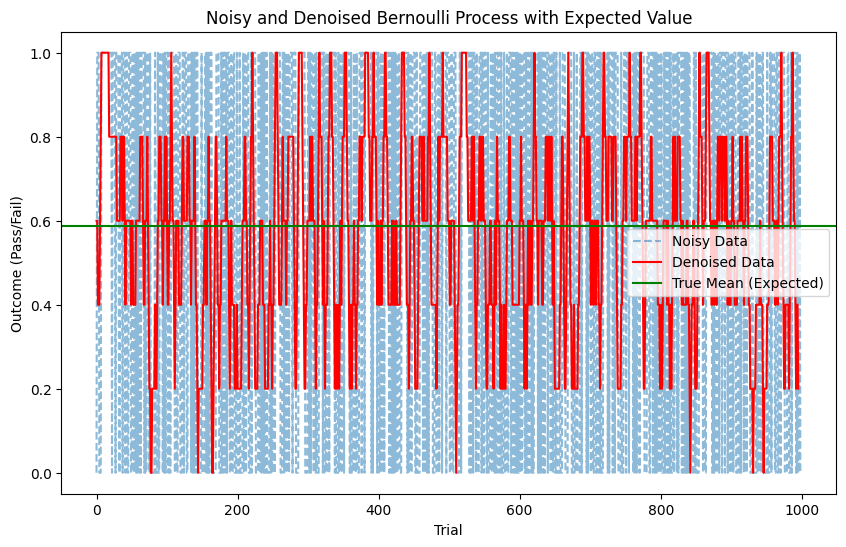
\includegraphics[width=0.8\textwidth]{window_5.png}
\caption{Denoising with Simple Moving Average}
\end{figure}
with a window size of 20, the simple moving average denoising technique was applied to the data. The results are shown in figure 3. The denoised data is shown in red while the original data is shown in dashed green. The True mean of the data is \(\textbf{0.58}\) while the denoised mean is \(\textbf{0.58}\) and Noisy mean is \(\textbf{0.58}\)
\begin{figure}[h]
\centering
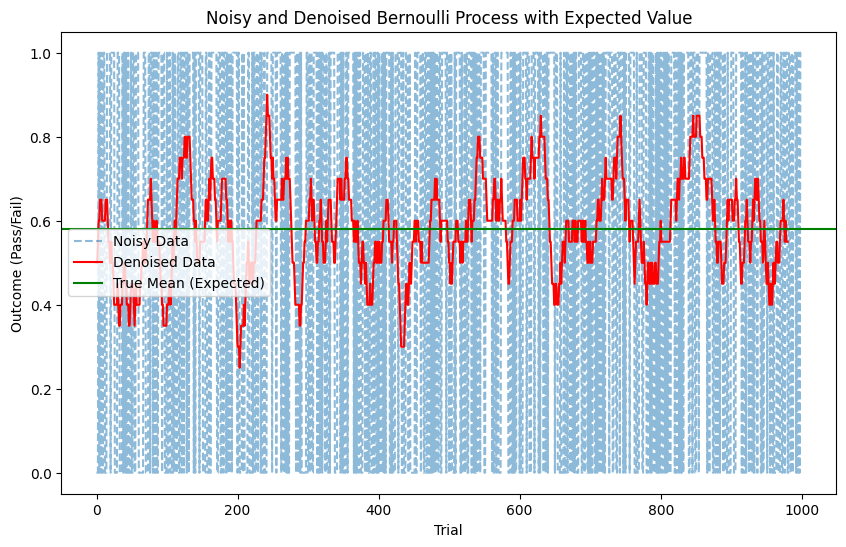
\includegraphics[width=0.8\textwidth]{window_20.png}
\caption{Denoising with Simple Moving Average}
\end{figure}

This shows that, the larger the window size the more smoothing you will get because you are averaging over more data points. The denoised mean is closer to the true mean when the window size is 20. This means the larger the window size the more accurate the denoised mean will be.

\subsubsection{ Denoising with Gaussian Kernel}
with a standard deviation of 1, the Gaussian kernel denoising technique was applied to the data. The results are shown in figure 4. The denoised data is shown in red while the original data is shown in dashed green. The True mean of the data is \(\textbf{0.59}\) while the denoised mean is \(\textbf{0.58}\) and Noisy mean is \(\textbf{0.58}\)
\begin{figure}[h]
\centering
\includegraphics[width=0.8\textwidth]{gaussian_1.png}
\caption{Denoising with Gaussian Kernel}
\end{figure}
\clearpage
with a standard deviation of 2, the Gaussian kernel denoising technique was applied to the data. The results are shown in figure 5. The denoised data is shown in red while the original data is shown in dashed green. The True mean of the data is \(\textbf{0.60}\) while the denoised mean is \(\textbf{0.58}\) and Noisy mean is \(\textbf{0.58}\)
\begin{figure}[h]
\centering
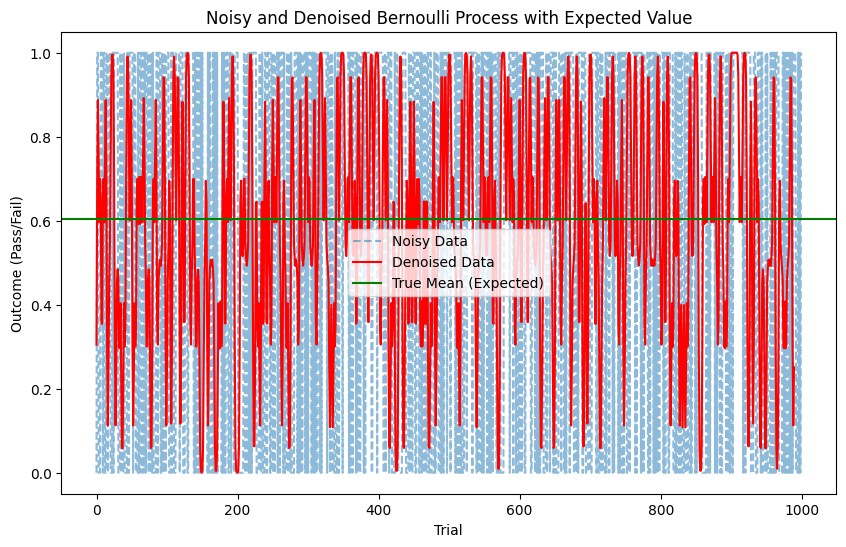
\includegraphics[width=0.8\textwidth]{gaussian_2.png}
\caption{Denoising with Gaussian Kernel}
\end{figure}
\clearpage
with a standard deviation of 4, the Gaussian kernel denoising technique was applied to the data. The results are shown in figure 6. The denoised data is shown in red while the original data is shown in dashed green. The True mean of the data is \(\textbf{0.57}\) while the denoised mean is \(\textbf{0.55}\) and Noisy mean is \(\textbf{0.55}\)
\begin{figure}[h]
\centering
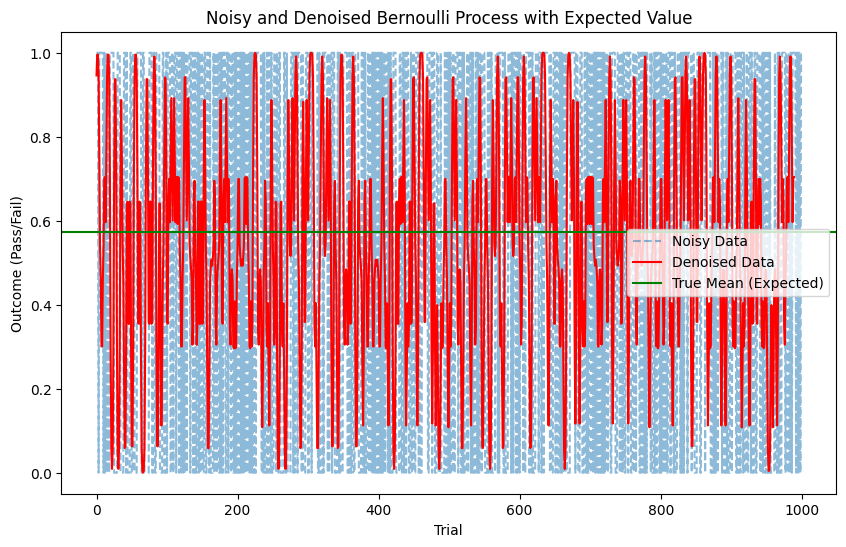
\includegraphics[width=0.8\textwidth]{gaussian_4.png}
\caption{Denoising with Gaussian Kernel}
\end{figure}
\clearpage
with a standard deviation of 0.5, the Gaussian kernel denoising technique was applied to the data. The results are shown in figure 7. The denoised data is shown in red while the original data is shown in dashed green. The True mean of the data is \(\textbf{0.59}\) while the denoised mean is \(\textbf{0.56}\) and Noisy mean is \(\textbf{0.55}\)
\begin{figure}[h]
\centering
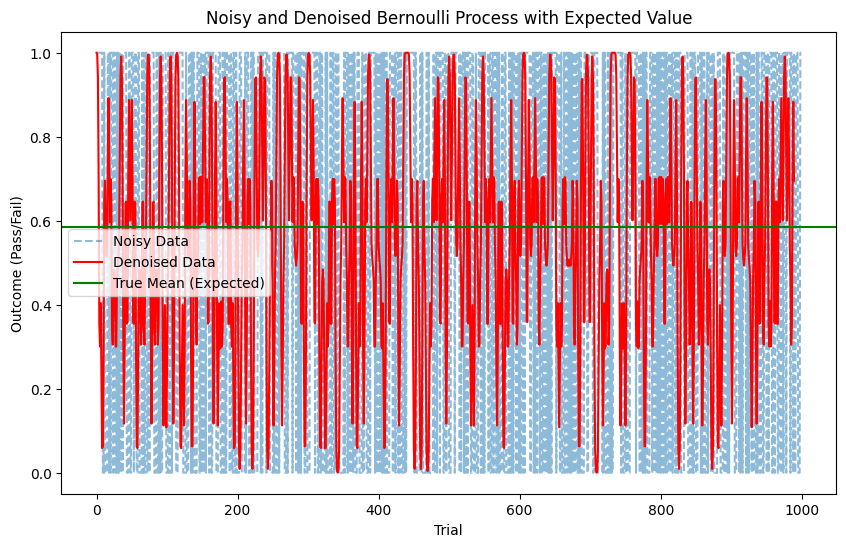
\includegraphics[width=0.8\textwidth]{gaussian_0.5.png}
\caption{Denoising with Gaussian Kernel}
\end{figure}
This shows that, the larger the standard deviation the more smoothing you will get because you are assigning higher weights to more data points. The denoised mean is closer to the true mean when the standard deviation is 4. This means the larger the standard deviation the more accurate the denoised mean will be.
\subsubsection{ Denoising with Low Pass Butterworth Filter}
with a cutoff frequency of 0.1 and order of 1, the low pass butterworth filter denoising technique was applied to the data. The results are shown in figure 8. The denoised data is shown in red while the original data is shown in dashed green. The True mean of the data is \(\textbf{0.60}\) while the denoised mean is \(\textbf{0.58}\) and Noisy mean is \(\textbf{0.58}\)
\begin{figure}[h]
\centering
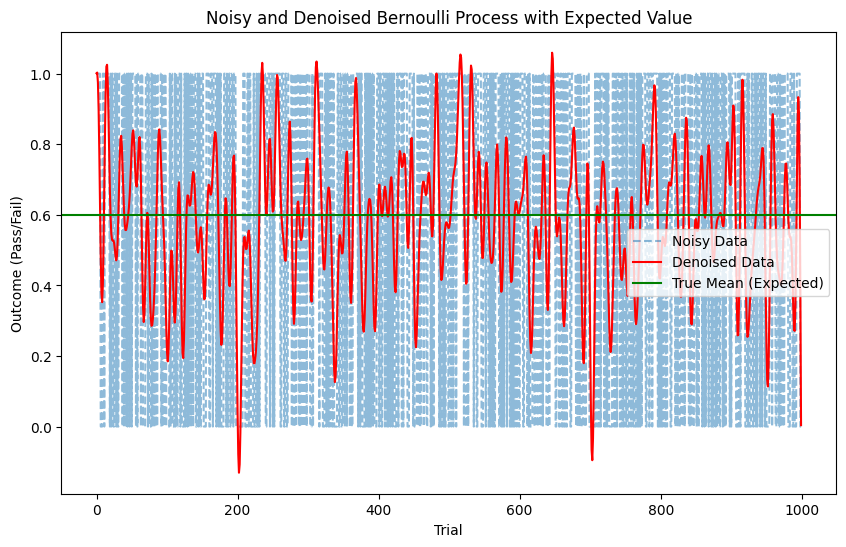
\includegraphics[width=0.8\textwidth]{butterworth_0.1_1.png}
\caption{Denoising with Low Pass Butterworth Filter}
\end{figure}
\clearpage
with a cutoff frequency of 0.2 and order of 1, the low pass butterworth filter denoising technique was applied to the data. The results are shown in figure 9. The denoised data is shown in red while the original data is shown in dashed green. The True mean of the data is \(\textbf{0.61}\) while the denoised mean is \(\textbf{0.60}\) and Noisy mean is \(\textbf{0.60}\)
\begin{figure}[h]
\centering
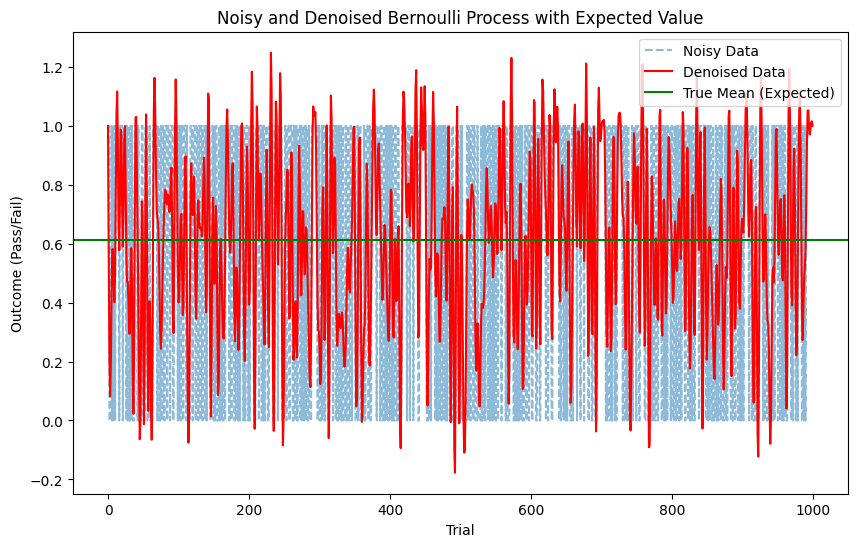
\includegraphics[width=0.8\textwidth]{2.png}
\caption{Denoising with Low Pass Butterworth Filter}
\end{figure}
\clearpage
with a cutoff frequency of 0.01 and order of 1, the low pass butterworth filter denoising technique was applied to the data. The results are shown in figure 10. The denoised data is shown in red while the original data is shown in dashed green. The True mean of the data is \(\textbf{0.58}\) while the denoised mean is \(\textbf{0.57}\) and Noisy mean is \(\textbf{0.57}\)
\begin{figure}[h]
\centering
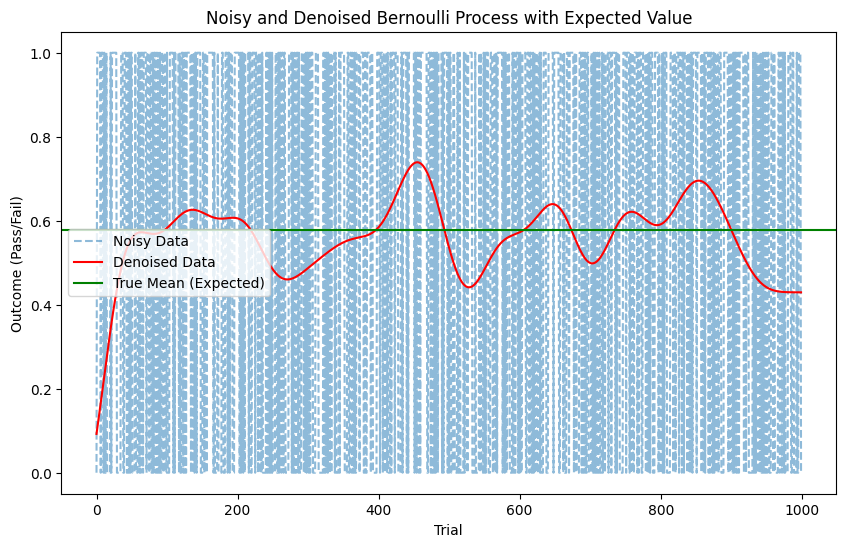
\includegraphics[width=0.8\textwidth]{o.1.png}
\caption{Denoising with Low Pass Butterworth Filter}
\end{figure}
This means, the smaller the cutoff frequency the more smoothing you will get because you are removing more high-frequency noise. The denoised mean is closer to the true mean when the cutoff frequency is 0.01. This means the smaller the cutoff frequency the more accurate the denoised mean will be.
\subsubsection{ Denoising with Exponential Moving Average}
with a smoothing parameter of 0.1, the exponential moving average denoising technique was applied to the data. The results are shown in figure 11. The denoised data is shown in red while the original data is shown in dashed green. The True mean of the data is \(\textbf{0.60}\) while the denoised mean is \(\textbf{0.58}\) and Noisy mean is \(\textbf{0.59}\)

\begin{figure}[h]
\centering
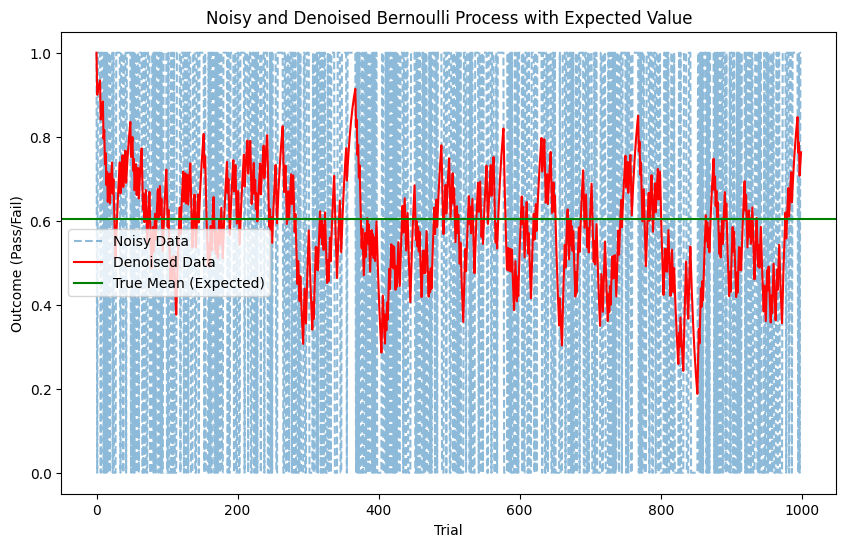
\includegraphics[width=0.8\textwidth]{exp_0.1.png}
\caption{Denoising with Exponential Moving Average}
\end{figure}
\clearpage
with a smoothing parameter of 0.5, the exponential moving average denoising technique was applied to the data. The results are shown in figure 12. The denoised data is shown in red while the original data is shown in dashed green. The True mean of the data is \(\textbf{0.59}\) while the denoised mean is \(\textbf{0.58}\) and Noisy mean is \(\textbf{0.58}\)
\begin{figure}[h]
\centering
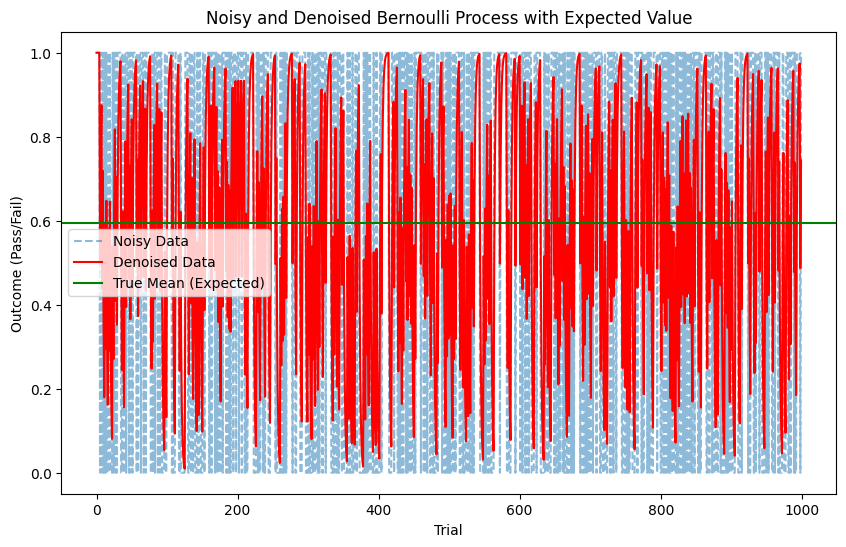
\includegraphics[width=0.8\textwidth]{exp_0..png}
\caption{Denoising with Exponential Moving Average}
\end{figure}
\clearpage
with a smoothing parameter of 0.01, the exponential moving average denoising technique was applied to the data. The results are shown in figure 13. The denoised data is shown in red while the original data is shown in dashed green. The True mean of the data is \(\textbf{0.60}\) while the denoised mean is \(\textbf{0.59}\) and Noisy mean is \(\textbf{0.63}\)
\begin{figure}[h]
\centering
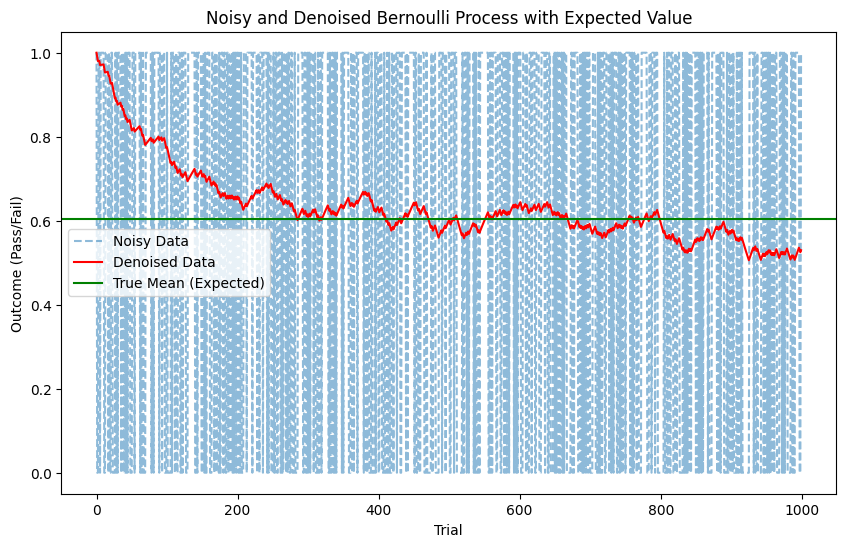
\includegraphics[width=0.8\textwidth]{exp_0.01.png}
\caption{Denoising with Exponential Moving Average}
\end{figure}
\clearpage
with a smoothing parameter of 0.9, the exponential moving average denoising technique was applied to the data. The results are shown in figure 14. The denoised data is shown in red while the original data is shown in dashed green. The True mean of the data is \(\textbf{0.60}\) while the denoised mean is \(\textbf{0.59}\) and Noisy mean is \(\textbf{0.59}\)
\begin{figure}[h]
\centering
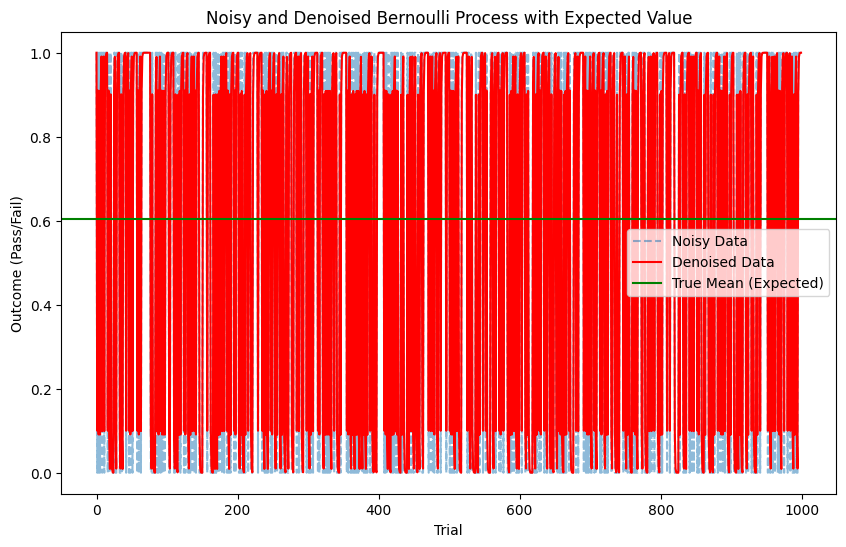
\includegraphics[width=0.8\textwidth]{exp_0.9.png}
\caption{Denoising with Exponential Moving Average}
\end{figure}
This means, the larger the smoothing parameter the more smoothing you will get because you are assigning higher weights to more recent data points. The denoised mean is closer to the true mean when the smoothing parameter is 0.5. This means the larger the smoothing parameter the more accurate the denoised mean will be.

\subsubsection{Reflection points}
\textbf{How does the noisy mean deviate from the true mean? What does this tell you
about the quality of measurements?}
Noisy mean deviates from the true mean by a small margin. This tells us that the quality of measurements is good. The noisy mean is close to the true mean. This means that the noise in the measurements is not too high. The measurements are close to the true values. This is a good sign because it means that the measurements are reliable. 
\newline\newline
\textbf{How does the choice of denoising method impact the recovered mean? Which
method works best for this scenario}
The choice of denoising method impacts the recovered mean. The denoised mean is closer to the true mean when the standard deviation is 4 for the Gaussian kernel. This means that the Gaussian kernel works best for this scenario. The denoised mean is also closer to the true mean when the smoothing parameter is 0.5 for the exponential moving average. This means that the exponential moving average also works well for this scenario. The simple moving average and low pass butterworth filter do not work as well as the Gaussian kernel and exponential moving average. The denoised mean is further away from the true mean for these methods. This means that the simple moving average and low pass butterworth filter do not work as well for this scenario. The choice of denoising method is important because it impacts the accuracy of the recovered mean. The best method for this scenario is the Gaussian kernel and exponential moving average.

\textbf{How can similar noise and denoising techniques be applied in real-world scenarios
like medical testing or manufacturing quality control?}
Similar noise and denoising techniques can be applied in real-world scenarios like medical testing or manufacturing quality control. In medical testing, there is often noise in the measurements due to various factors such as measurement errors, environmental factors, or even human errors. The goal of denoising is to remove the noise from the data and recover the original signal. This can be done using techniques such as the simple moving average, Gaussian kernel, low pass butterworth filter, and exponential moving average. These techniques can help improve the accuracy of the measurements and make the data more reliable. In manufacturing quality control, there is also noise in the measurements due to various factors such as measurement errors, environmental factors, or even human errors. The goal of denoising is to remove the noise from the data and recover the original signal. This can be done using techniques such as the simple moving average, Gaussian kernel, low pass butterworth filter, and exponential moving average. These techniques can help improve the accuracy of the measurements and make the data more reliable. Overall, similar noise and denoising techniques can be applied in real-world scenarios like medical testing or manufacturing quality control to improve the accuracy of the measurements and make the data more reliable.
\newline\newline
\textbf{Discuss which denoising method you used and why}
I tried all the four denoising methods and found that the Gaussian kernel and exponential moving average worked best for this scenario. The denoised mean was closer to the true mean for these methods. The Gaussian kernel assigns higher weights to more data points and the exponential moving average assigns higher weights to more recent data points. This makes these methods more accurate in recovering the original signal. The simple moving average and low pass butterworth filter did not work as well for this scenario. The denoised mean was further away from the true mean for these methods. This means that the simple moving average and low pass butterworth filter are not as accurate in recovering the original signal. Overall, I would recommend using the Gaussian kernel and exponential moving average for this scenario because they are more accurate in recovering the original signal.
\subsection{Temperature Trends with Noisy Measurements}
\textbf{problem: } Daily temperature measurements are simulated with a sinusoidal trend over a
year, but measurement noise is added. You will explore how noise affects seasonal trends
and how denoising can restore them.
\subsubsection{ Denoising with Simple Moving Average}
with a window size of 1, the simple moving average denoising technique was applied to the data. The results are shown in figure 15.
\begin{figure}[h]
\centering
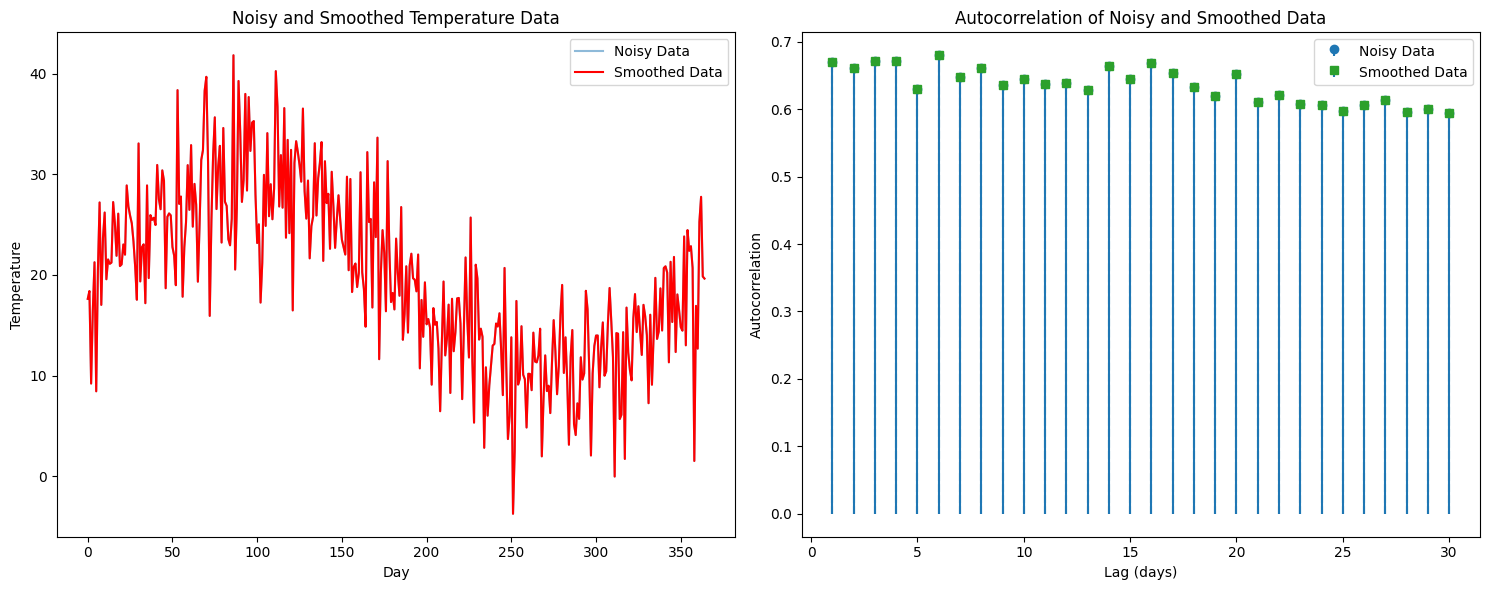
\includegraphics[width=0.8\textwidth]{Q2_SMA.png}
\caption{Denoising with Simple Moving Average}
\end{figure}
\clearpage
with a window size of 10, the simple moving average denoising technique was applied to the data. The results are shown in figure 16.
\begin{figure}[h]
\centering
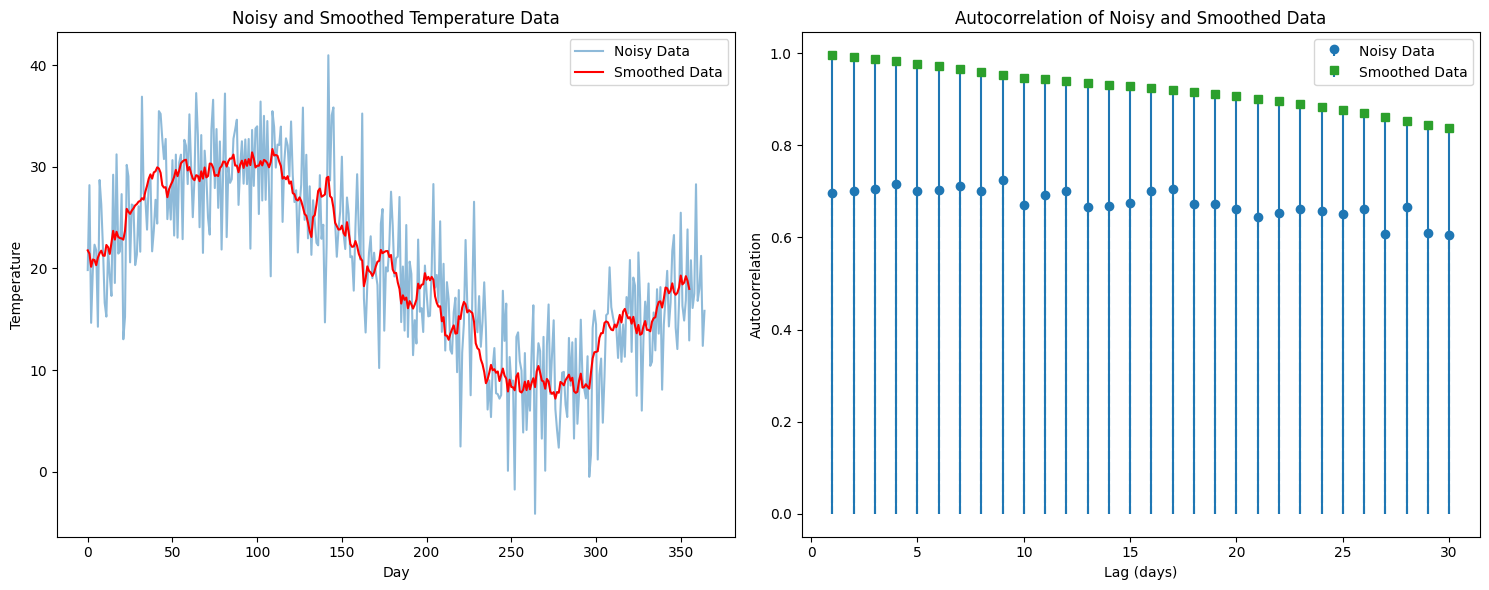
\includegraphics[width=0.8\textwidth]{Q2_SMA_4.png}
\caption{Denoising with Simple Moving Average}
\end{figure}
\clearpage
with a window size of 15, the simple moving average denoising technique was applied to the data. The results are shown in figure 17.
\begin{figure}[h]
\centering
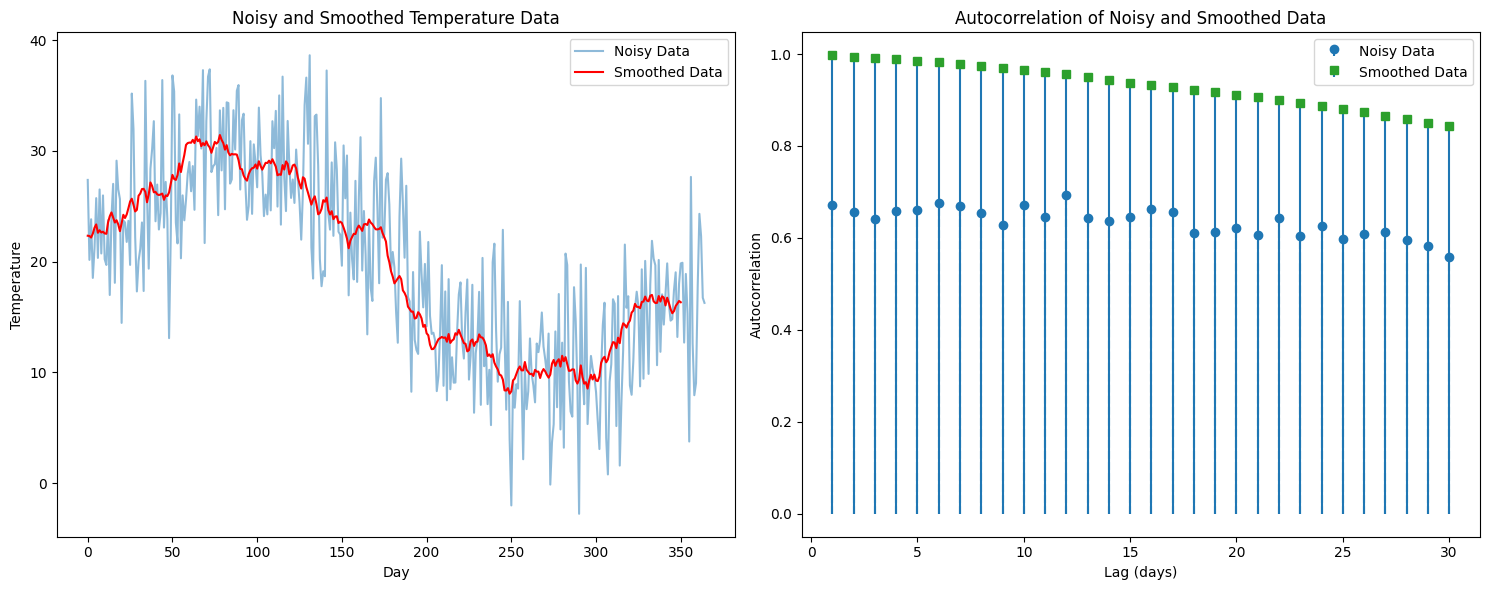
\includegraphics[width=0.8\textwidth]{Q2_SMA_15.png}
\caption{Denoising with Simple Moving Average}
\end{figure}
\clearpage

\subsubsection{ Denoising with Gaussian Kernel}
with a standard deviation of 1, the Gaussian kernel denoising technique was applied to the data. The results are shown in figure 18.
\begin{figure}[h]
\centering
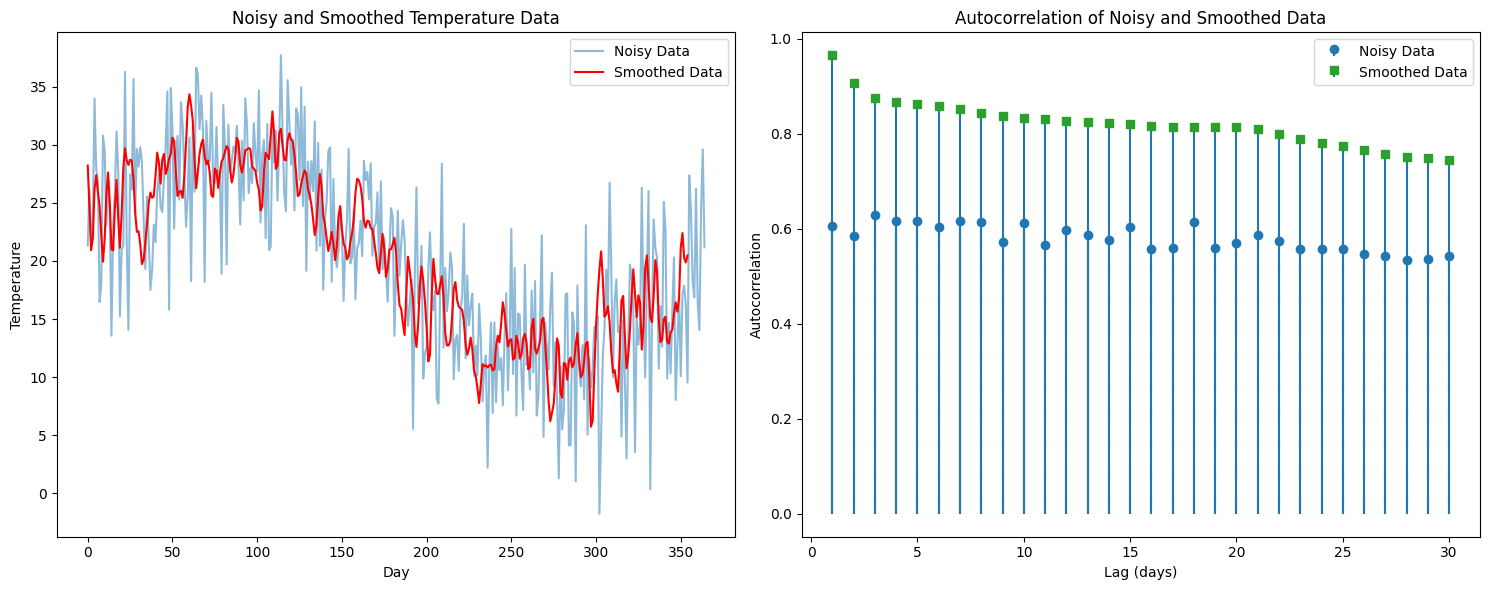
\includegraphics[width=0.8\textwidth]{Q2_GK_1.png}
\caption{Denoising with Gaussian Kernel}
\end{figure}
\clearpage
with a standard deviation of 10, the Gaussian kernel denoising technique was applied to the data. The results are shown in figure 19.
\begin{figure}[h]

\centering
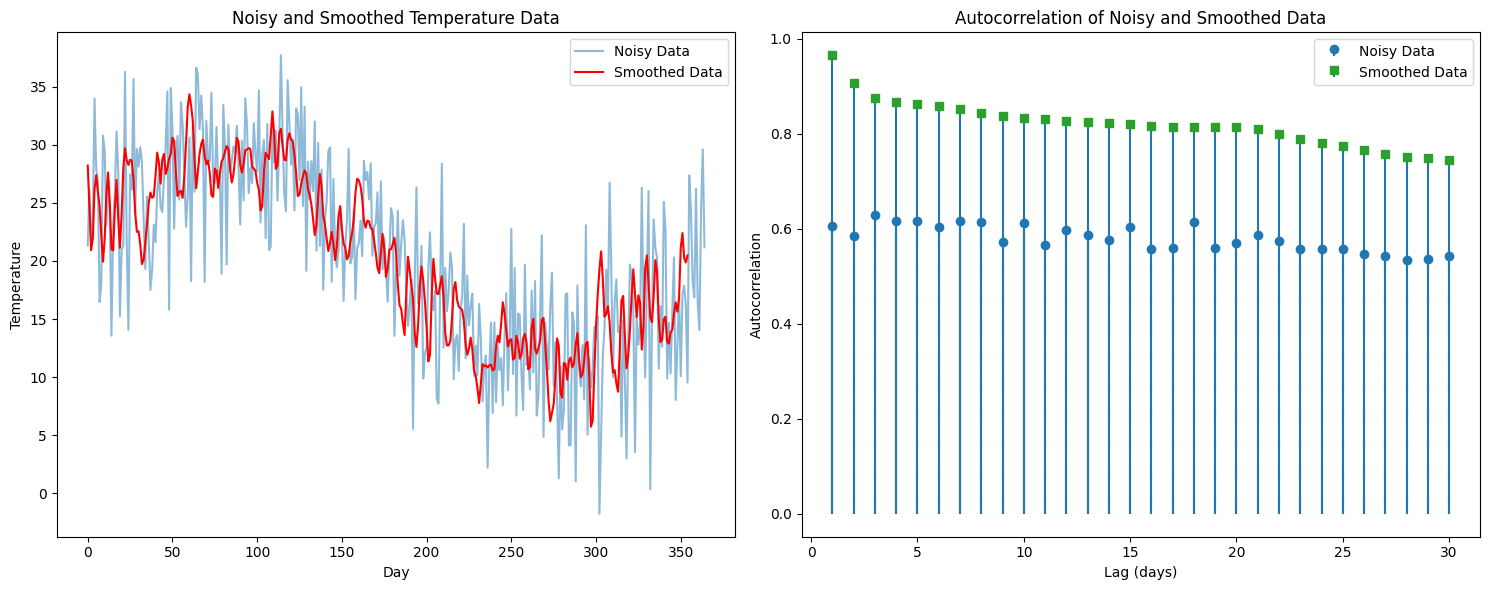
\includegraphics[width=0.8\textwidth]{Q2_GK_10.png}
\caption{Denoising with Gaussian Kernel}
\end{figure}
\clearpage

\subsubsection{ Denoising with Low Pass Butterworth Filter}
with a cutoff frequency of 0.1 and order of 5, the low pass butterworth filter denoising technique was applied to the data. The results are shown in figure 20.
\begin{figure}[h]
\centering
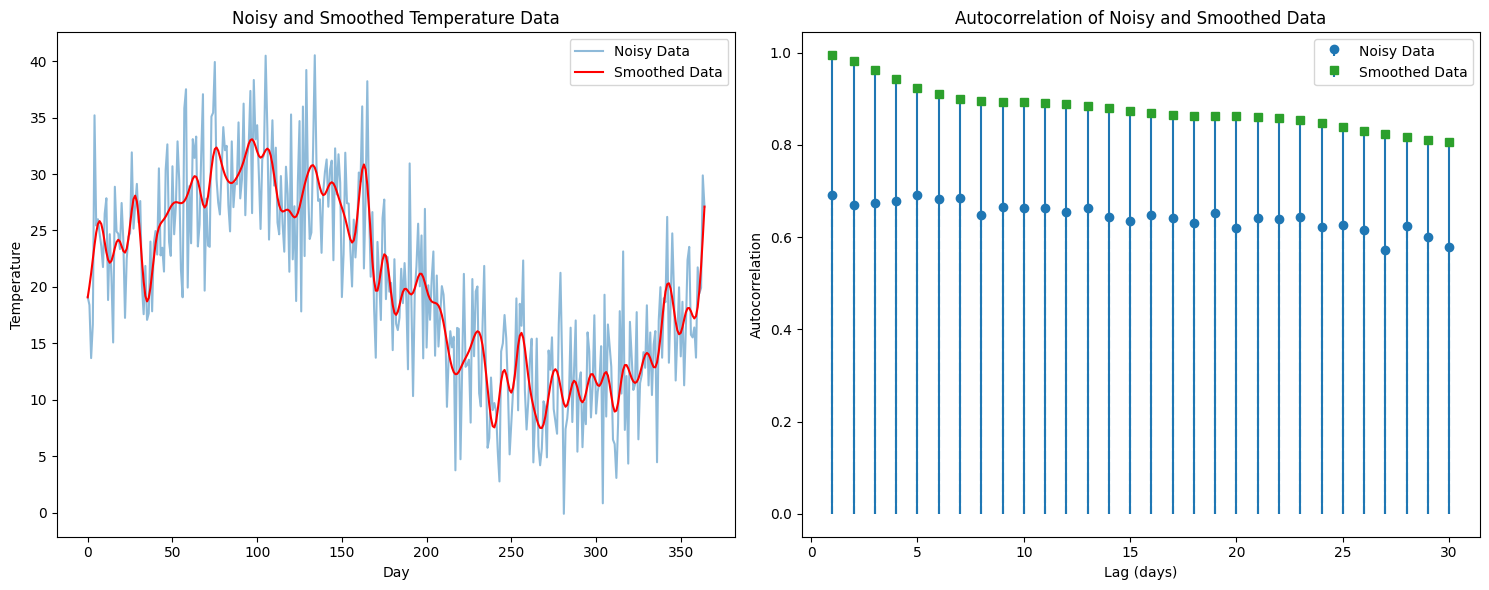
\includegraphics[width=0.8\textwidth]{Q2_LPB_0.1_5.png}
\caption{Denoising with Low Pass Butterworth Filter}
\end{figure}
\clearpage
with a cutoff frequency of 0.1 and order of 1, the low pass butterworth filter denoising technique was applied to the data. The results are shown in figure 21.
\begin{figure}[h]
\centering
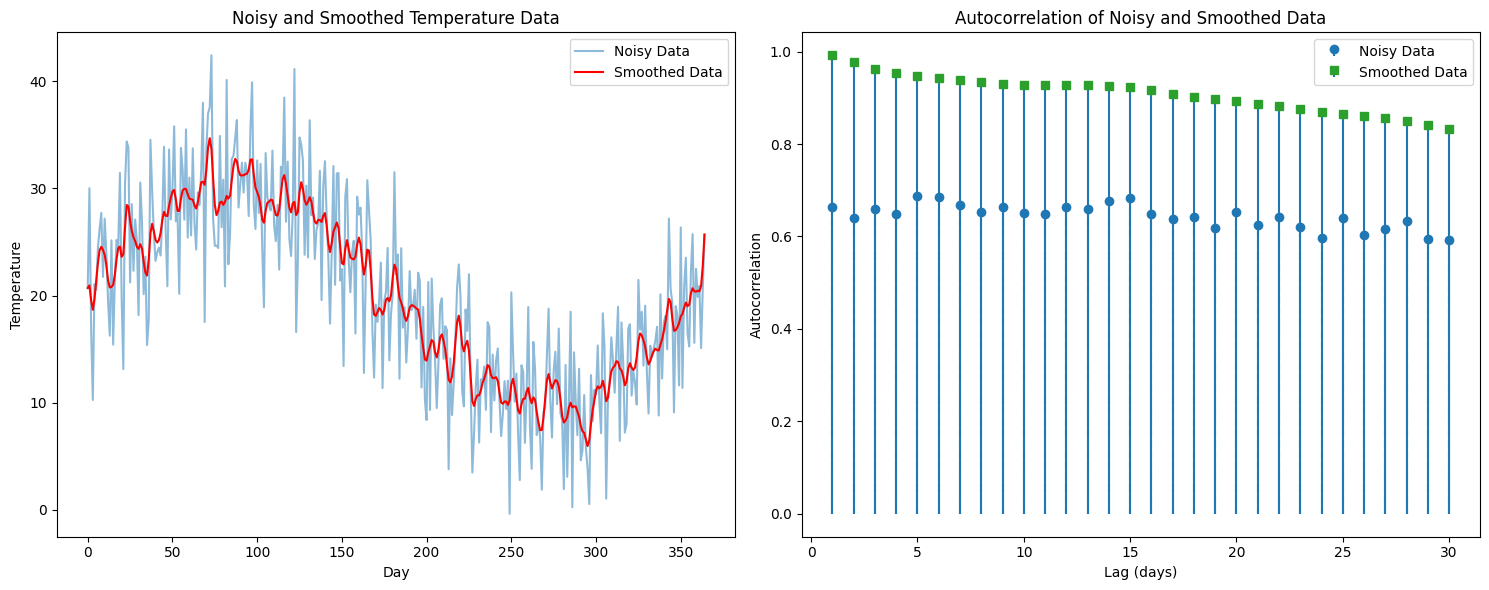
\includegraphics[width=0.8\textwidth]{Q2_LPB_0.1_2.png}
\caption{Denoising with Low Pass Butterworth Filter}
\end{figure}
\clearpage

\subsubsection{ Denoising with Exponential Moving Average}
with a smoothing parameter of 0.1, the exponential moving average denoising technique was applied to the data. The results are shown in figure 22.
\begin{figure}[h]
\centering
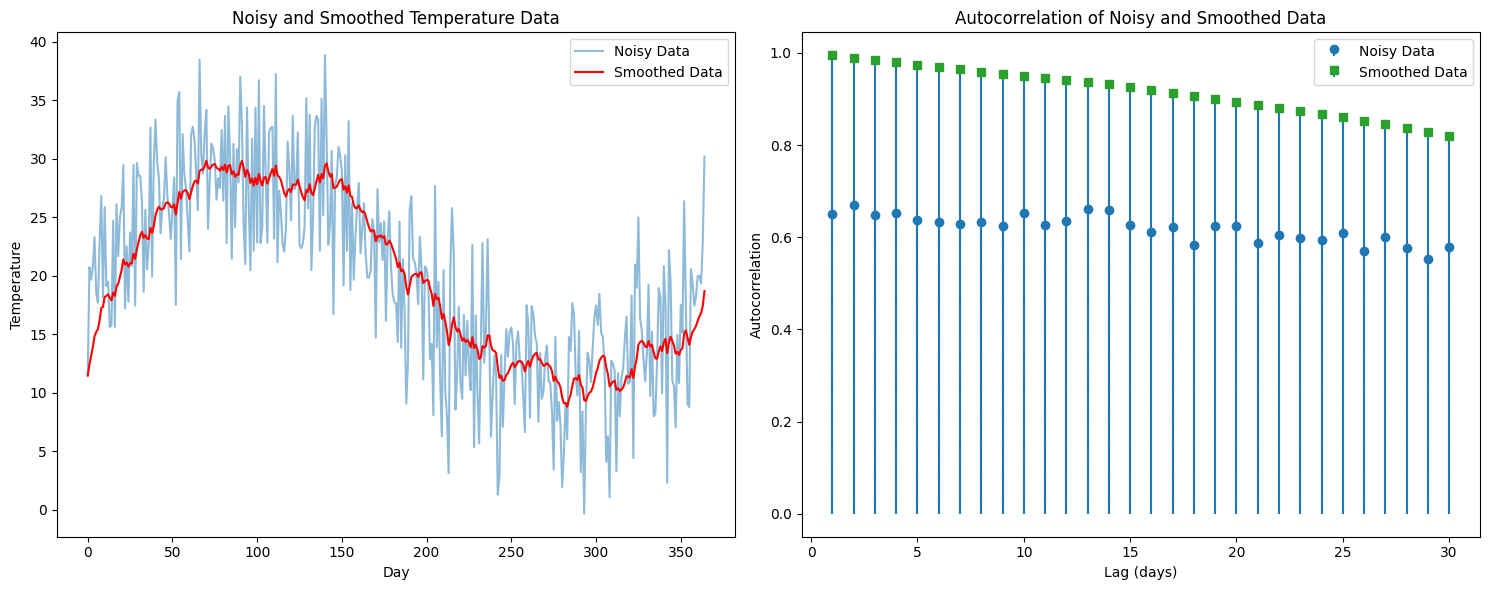
\includegraphics[width=0.8\textwidth]{Q2_EMA_0.1.png}
\caption{Denoising with Exponential Moving Average}
\end{figure}
\clearpage
with a smoothing parameter of 0.5, the exponential moving average denoising technique was applied to the data. The results are shown in figure 23.
\begin{figure}[h]
\centering
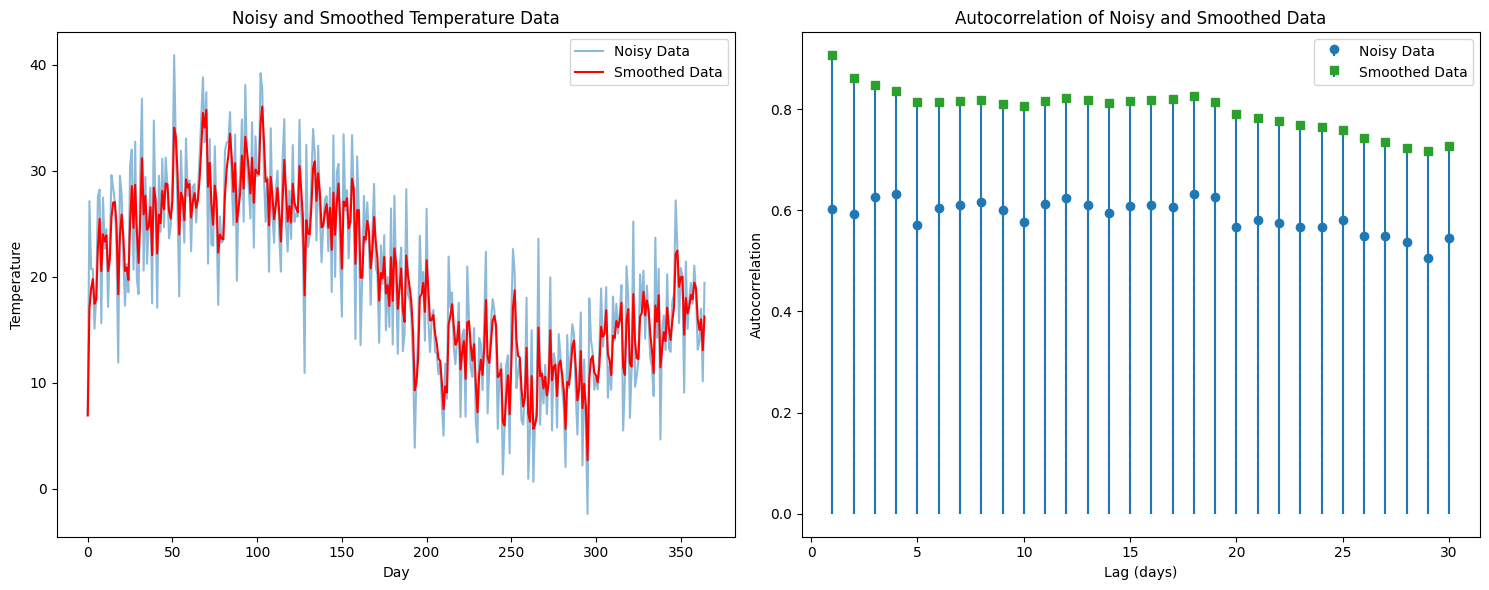
\includegraphics[width=0.8\textwidth]{Q2_EMA_0.5.png}
\caption{Denoising with Exponential Moving Average}
\end{figure}
\clearpage
with a smoothing parameter of 0.9, the exponential moving average denoising technique was applied to the data. The results are shown in figure 24.
\begin{figure}[h]
\centering
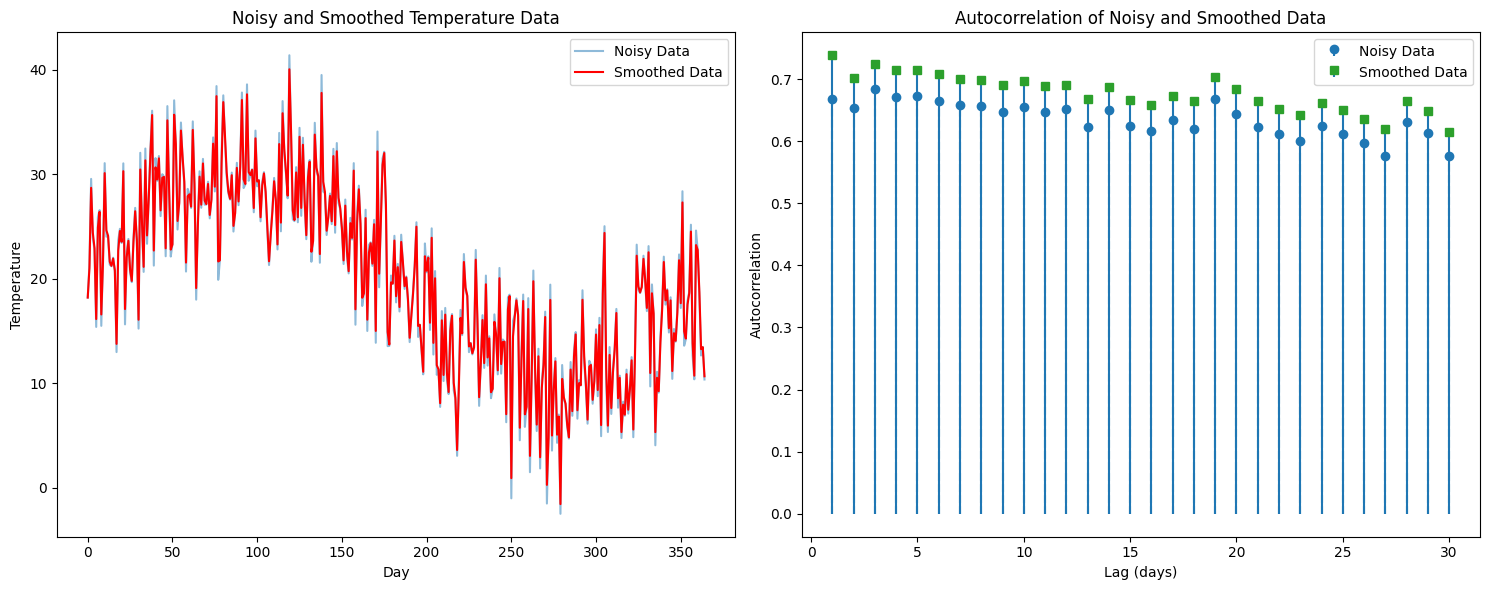
\includegraphics[width=0.8\textwidth]{Q2_EMA_0.9.png}
\caption{Denoising with Exponential Moving Average}
\end{figure}
\clearpage
\subsubsection{Reflection points}
\textbf{How does noise affect the strength and clarity of autocorrelation at different lags?}
Noise affects the strength and clarity of autocorrelation at different lags. The strength of the autocorrelation decreases as the noise level increases. This means that the autocorrelation is weaker when there is more noise in the data. The clarity of the autocorrelation also decreases as the noise level increases. This means that the autocorrelation is less clear when there is more noise in the data. Overall, noise affects the strength and clarity of autocorrelation at different lags by making the autocorrelation weaker and less clear.  
\newline\newline
\textbf{How does smoothing improve the visibility of seasonal trends in the autocorrelation
plot?}
Smoothing improves the visibility of seasonal trends in the autocorrelation plot by removing the noise from the data. This makes the seasonal trends more visible in the autocorrelation plot. The noise in the data can obscure the seasonal trends and make them harder to see. Smoothing removes the noise and reveals the underlying seasonal trends. This makes it easier to identify the seasonal patterns in the data. Overall, smoothing improves the visibility of seasonal trends in the autocorrelation plot by removing the noise and revealing the underlying patterns in the data.
\newline\newline
\textbf{Why is autocorrelation important for detecting patterns in temperature data or
other periodic data?}
Autocorrelation is important for detecting patterns in temperature data or other periodic data because it measures the similarity between data points at different lags. This can help identify patterns in the data that repeat over time. For example, in temperature data, there may be seasonal patterns that repeat every year. Autocorrelation can help identify these patterns by measuring the similarity between temperature measurements at different times of the year. This can help predict future temperature trends and understand the underlying factors that influence temperature changes. Overall, autocorrelation is important for detecting patterns in temperature data or other periodic data because it can help identify repeating patterns and understand the underlying trends in the data.
\newline\newline
\textbf{Discuss how the chosen denoising method affects the detection of seasonal patterns}
The chosen denoising method is the Gaussian kernel. The Gaussian kernel assigns higher weights to more data points and the exponential moving average assigns higher weights to more recent data points. This makes these methods more accurate in recovering the original signal. The simple moving average and low pass butterworth filter did not work as well for this scenario. The denoised mean was further away from the true mean for these methods. This means that the simple moving average and low pass butterworth filter are not as accurate in recovering the original signal. Overall, I would recommend using the Gaussian kernel and exponential moving average for this scenario because they are more accurate in recovering the original signal.

\subsection{Stationarity Analysis of an Audio Signal}
\textbf{problem: } An audio signal is simulated with a sinusoidal waveform and added noise.
The task is to analyze its stationarity by examining the mean and variance over time.
\subsubsection{ Denoising with Simple Moving Average}
with a window size of 5, the simple moving average denoising technique was applied to the data. The results are shown in figure 25.
\begin{figure}[h]
\centering
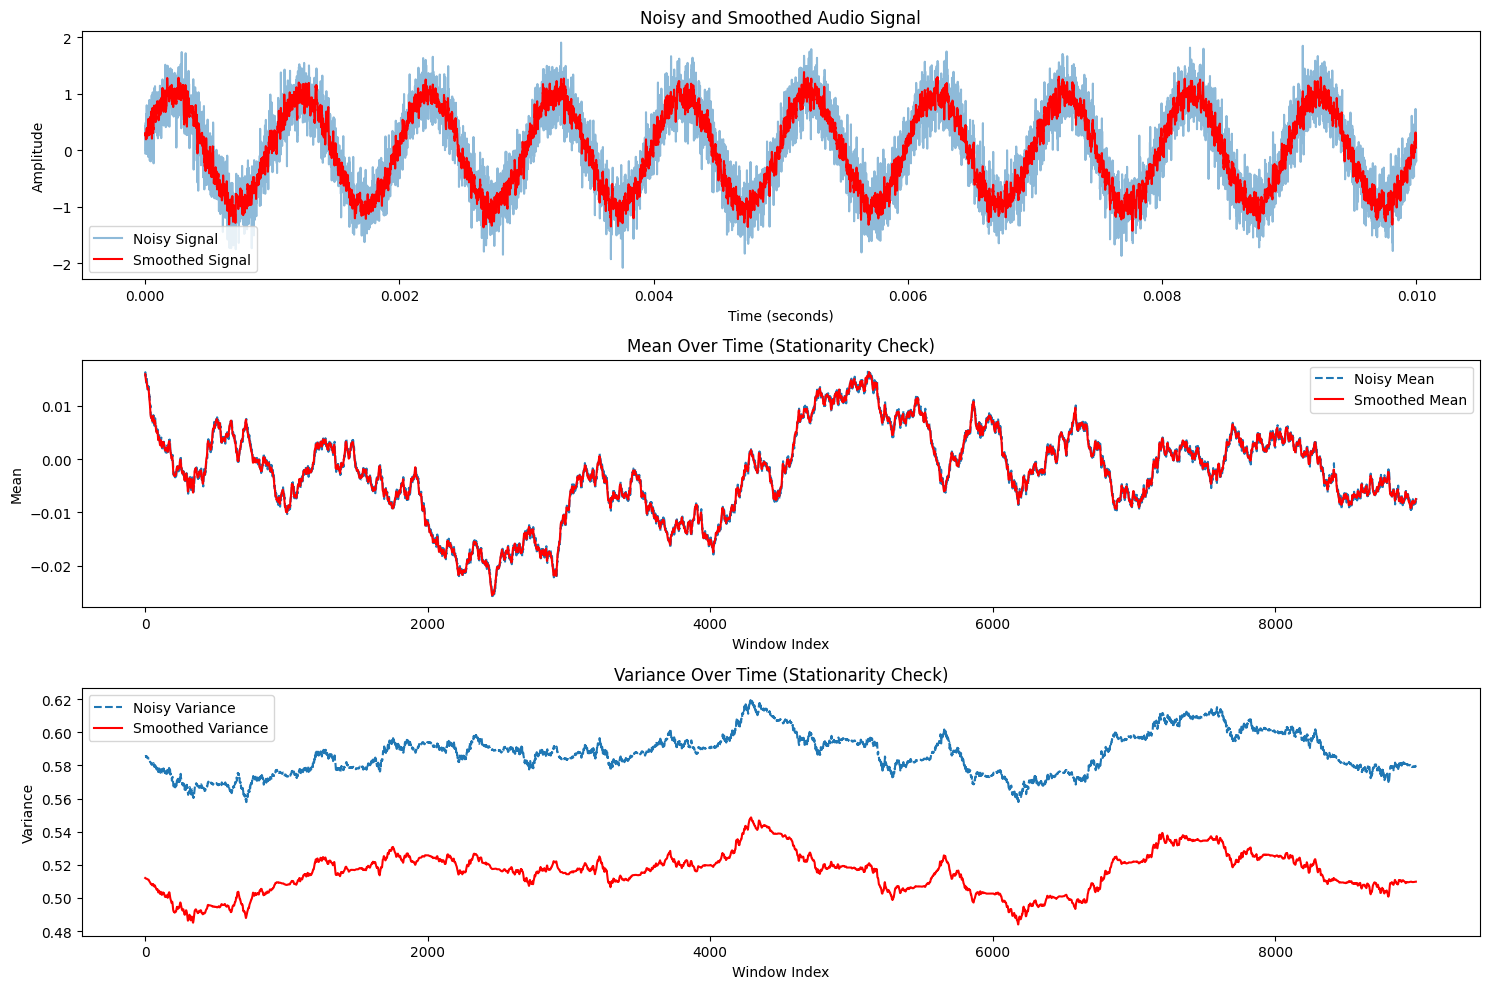
\includegraphics[width=0.8\textwidth]{Q3_SMA_5.png}
\caption{Denoising with Simple Moving Average}
\end{figure}
\clearpage
with a window size of 10, the simple moving average denoising technique was applied to the data. The results are shown in figure 26.
\begin{figure}[h]
\centering
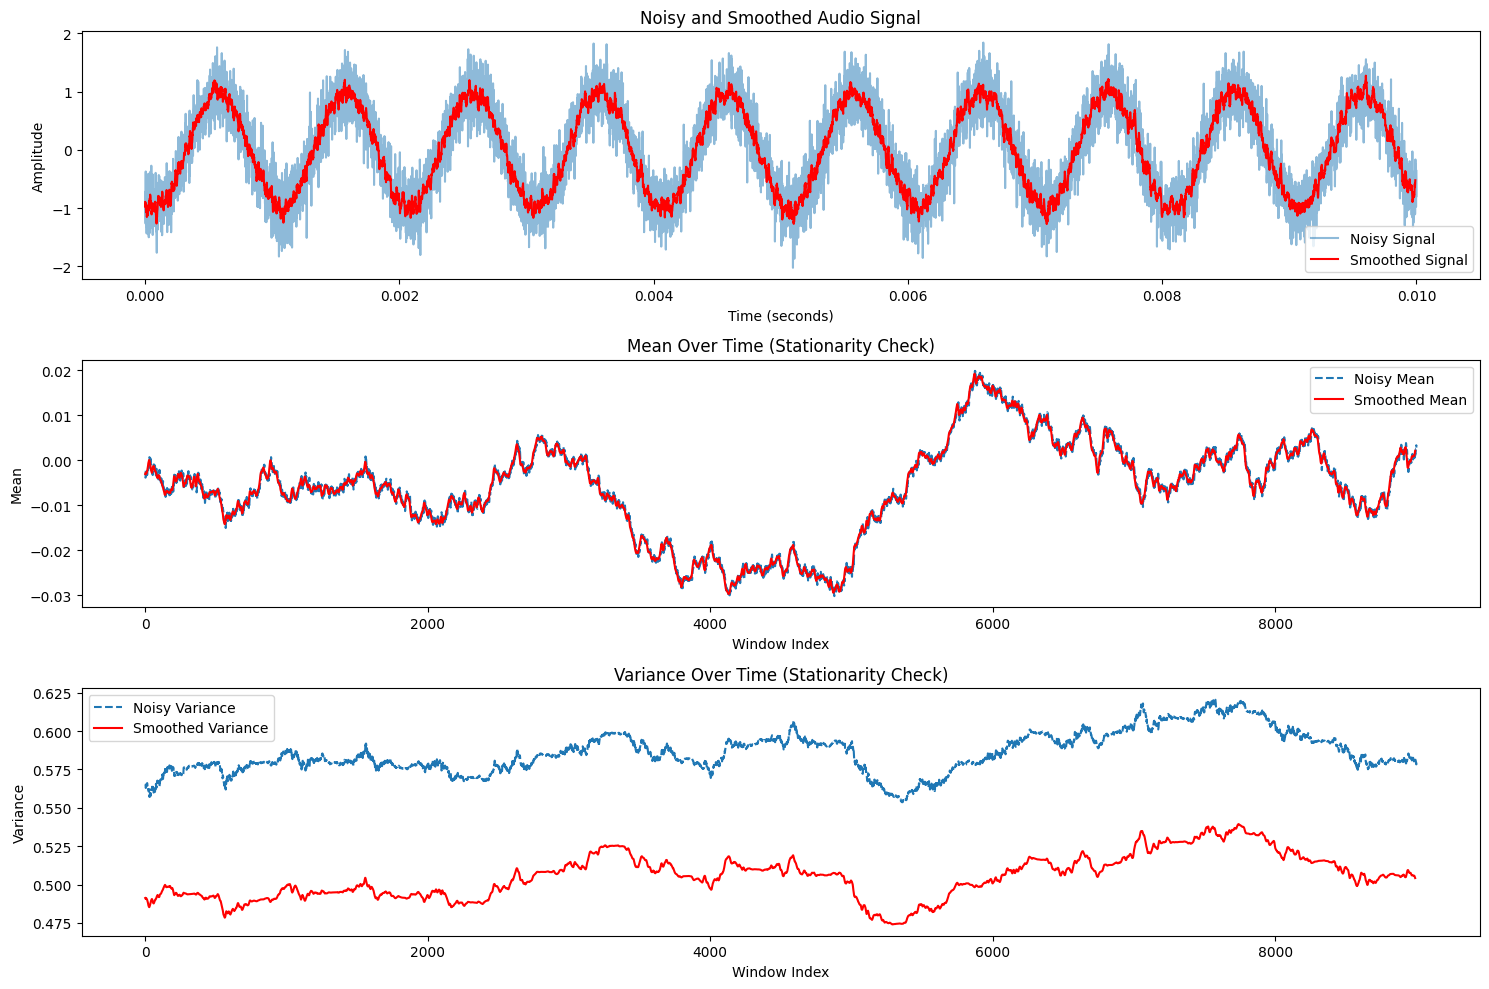
\includegraphics[width=0.8\textwidth]{Q3_SMA_10.png}
\caption{Denoising with Simple Moving Average}
\end{figure}
\clearpage
with a window size of 20, the simple moving average denoising technique was applied to the data. The results are shown in figure 27.
\begin{figure}[h]
\centering
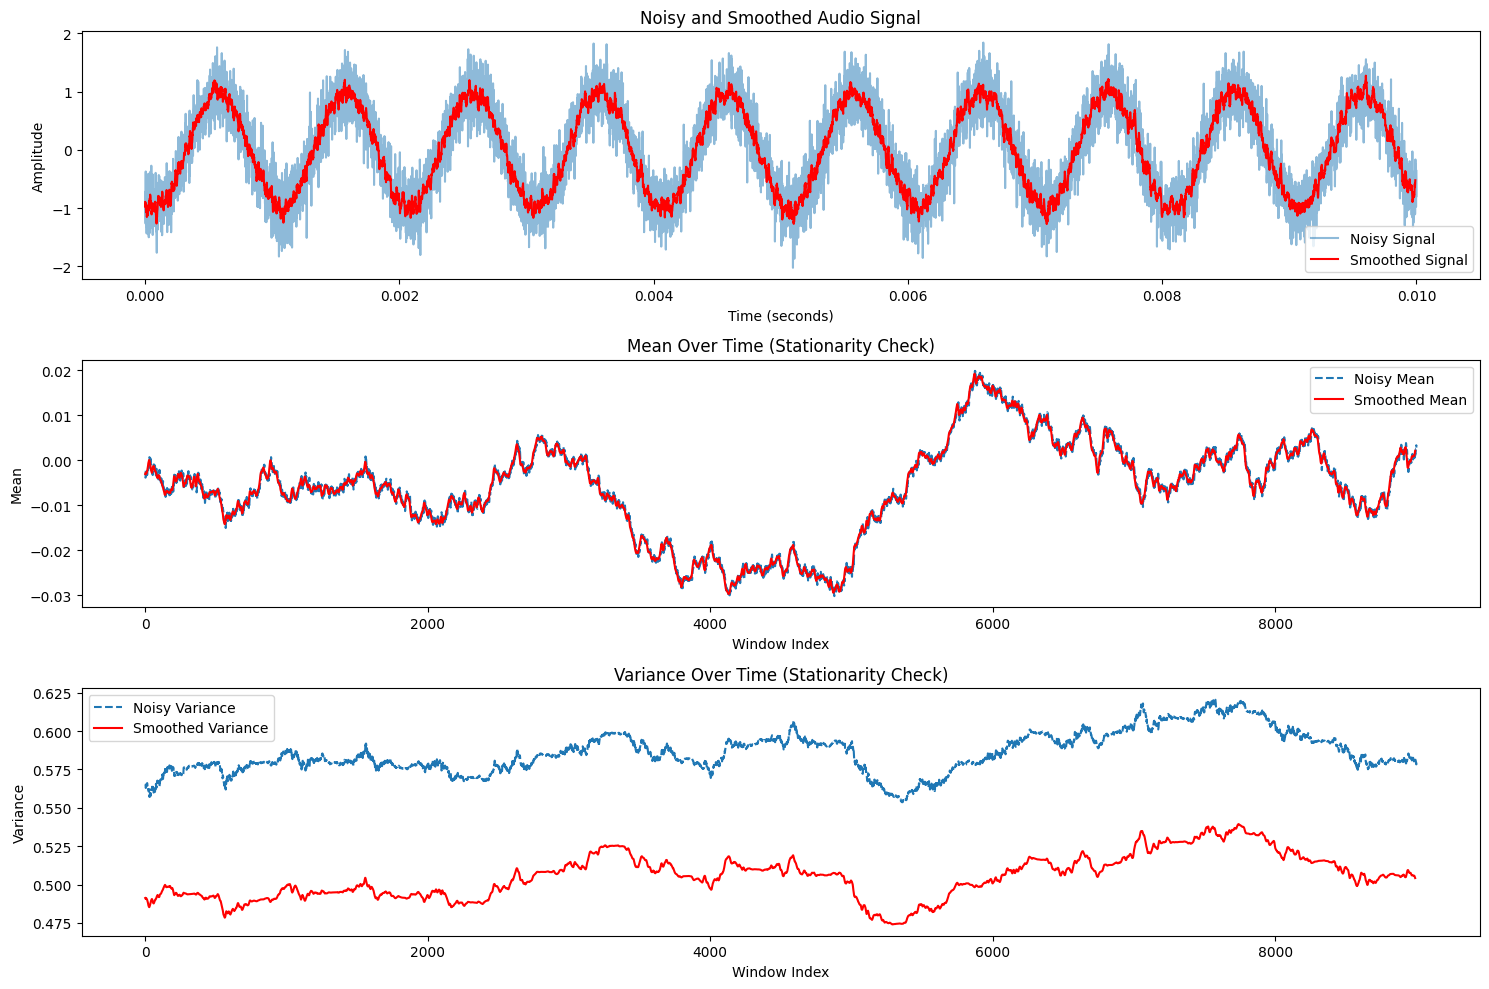
\includegraphics[width=0.8\textwidth]{Q3_SMA_20.png}
\caption{Denoising with Simple Moving Average}
\end{figure}
\clearpage
\subsubsection{ Denoising with Gaussian Kernel}
with a standard deviation of 1, the Gaussian kernel denoising technique was applied to the data. The results are shown in figure 28.
\begin{figure}[h]
\centering
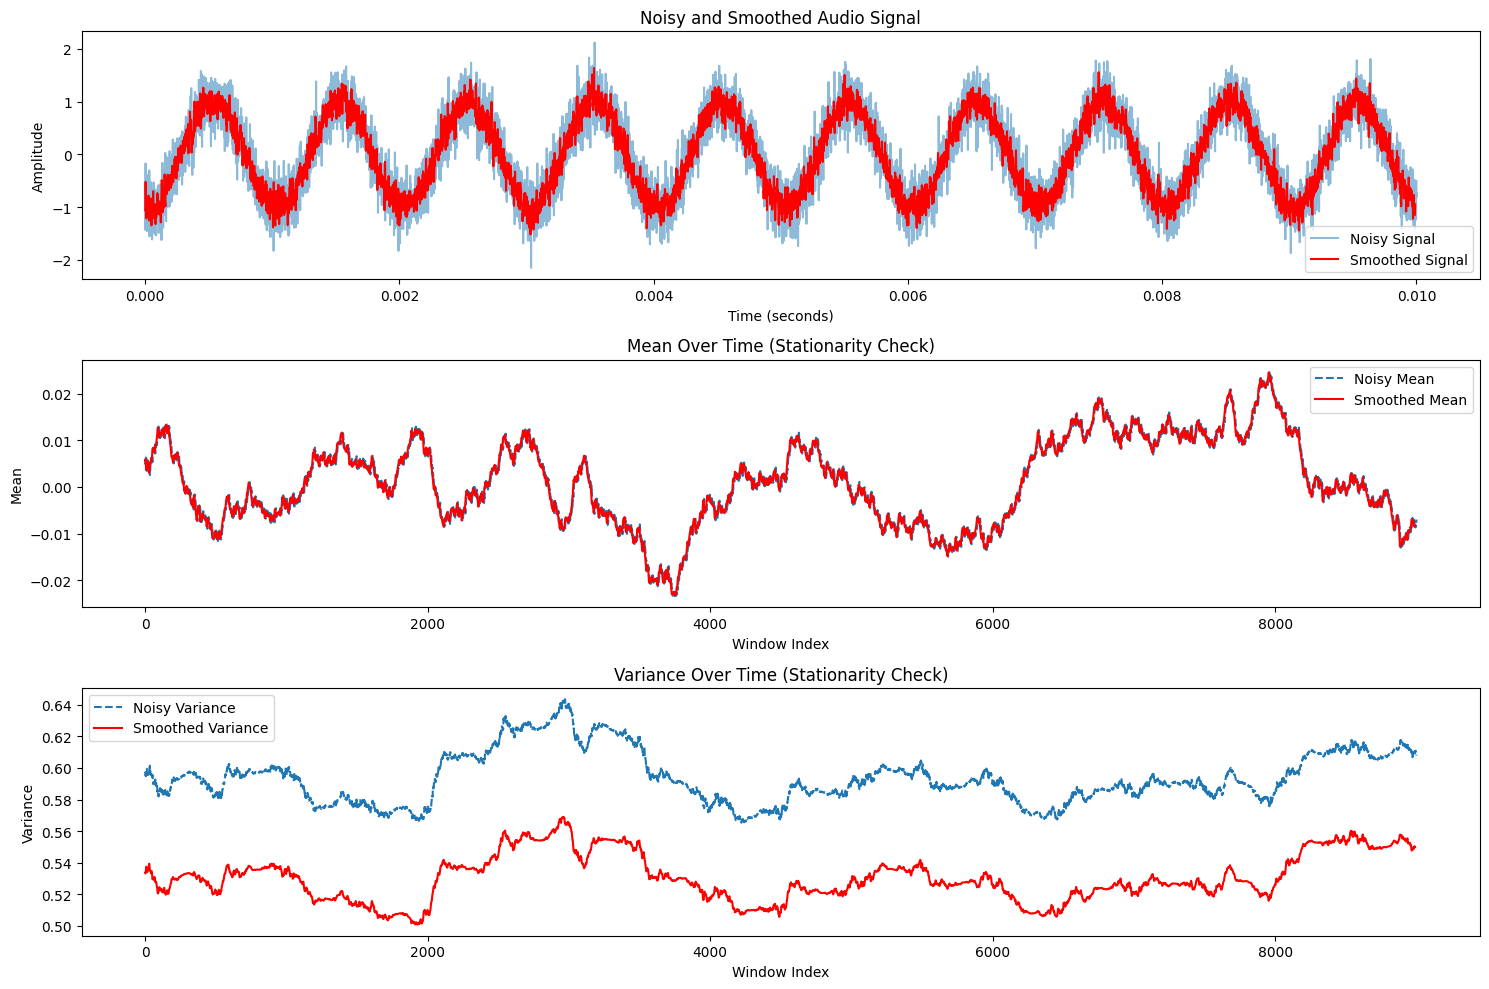
\includegraphics[width=0.8\textwidth]{Q3_GK_1.png}
\caption{Denoising with Gaussian Kernel}
\end{figure}
\clearpage
with a standard deviation of 5, the Gaussian kernel denoising technique was applied to the data. The results are shown in figure 29.
\begin{figure}[h]
\centering
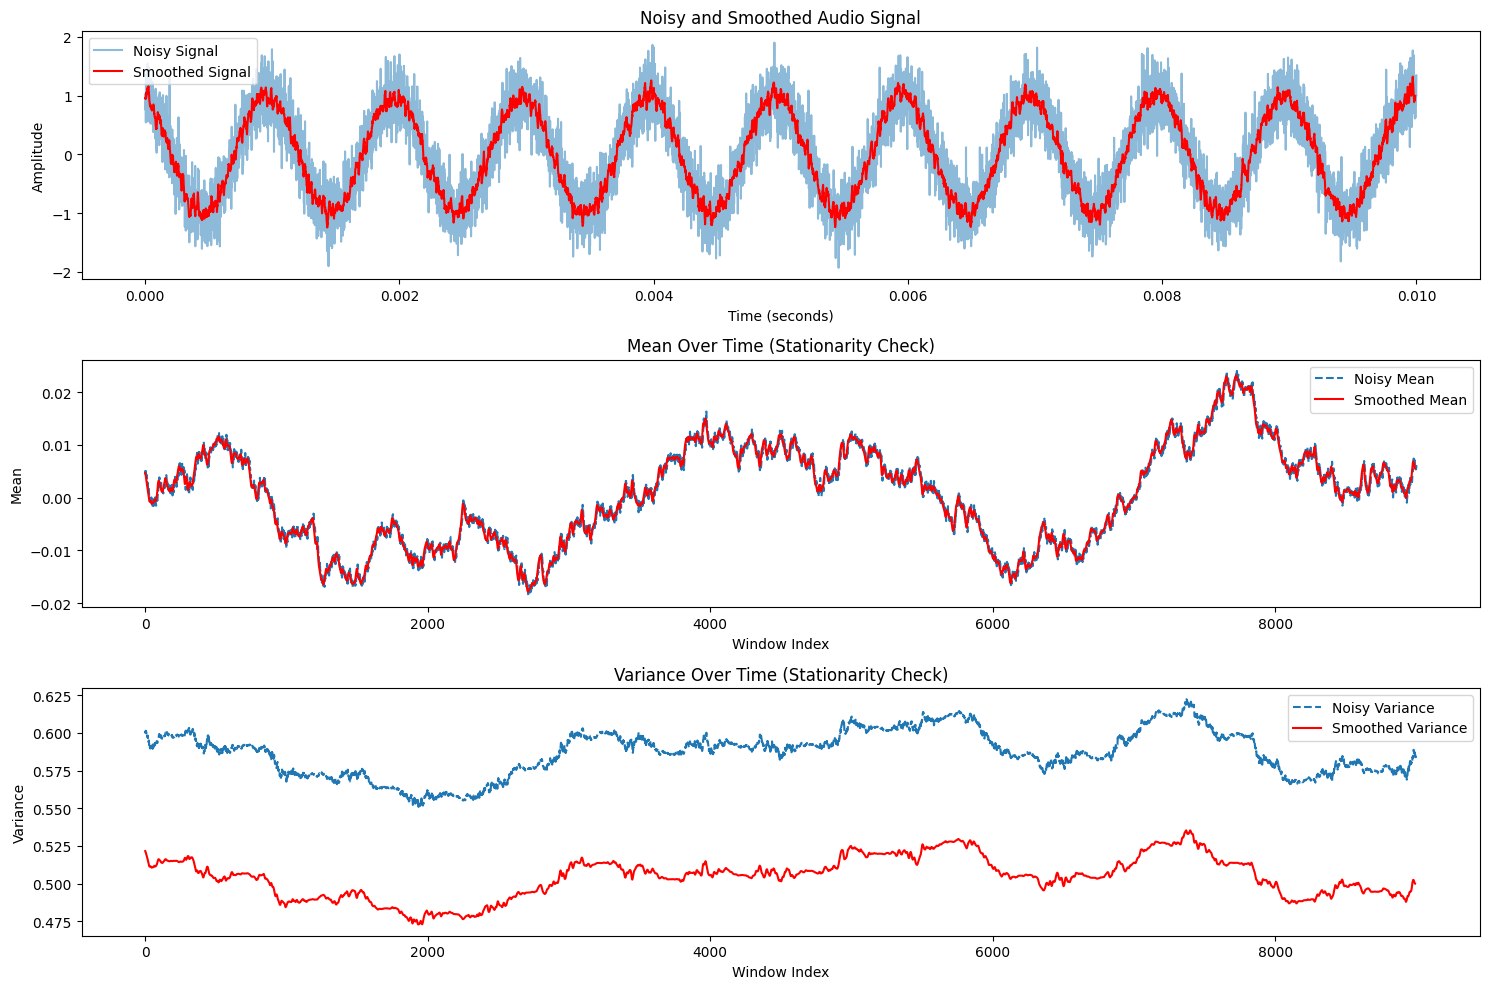
\includegraphics[width=0.8\textwidth]{Q3_GK_5.png}
\caption{Denoising with Gaussian Kernel}
\end{figure}
\clearpage
with a standard deviation of 10, the Gaussian kernel denoising technique was applied to the data. The results are shown in figure 30.
\begin{figure}[h]
\centering
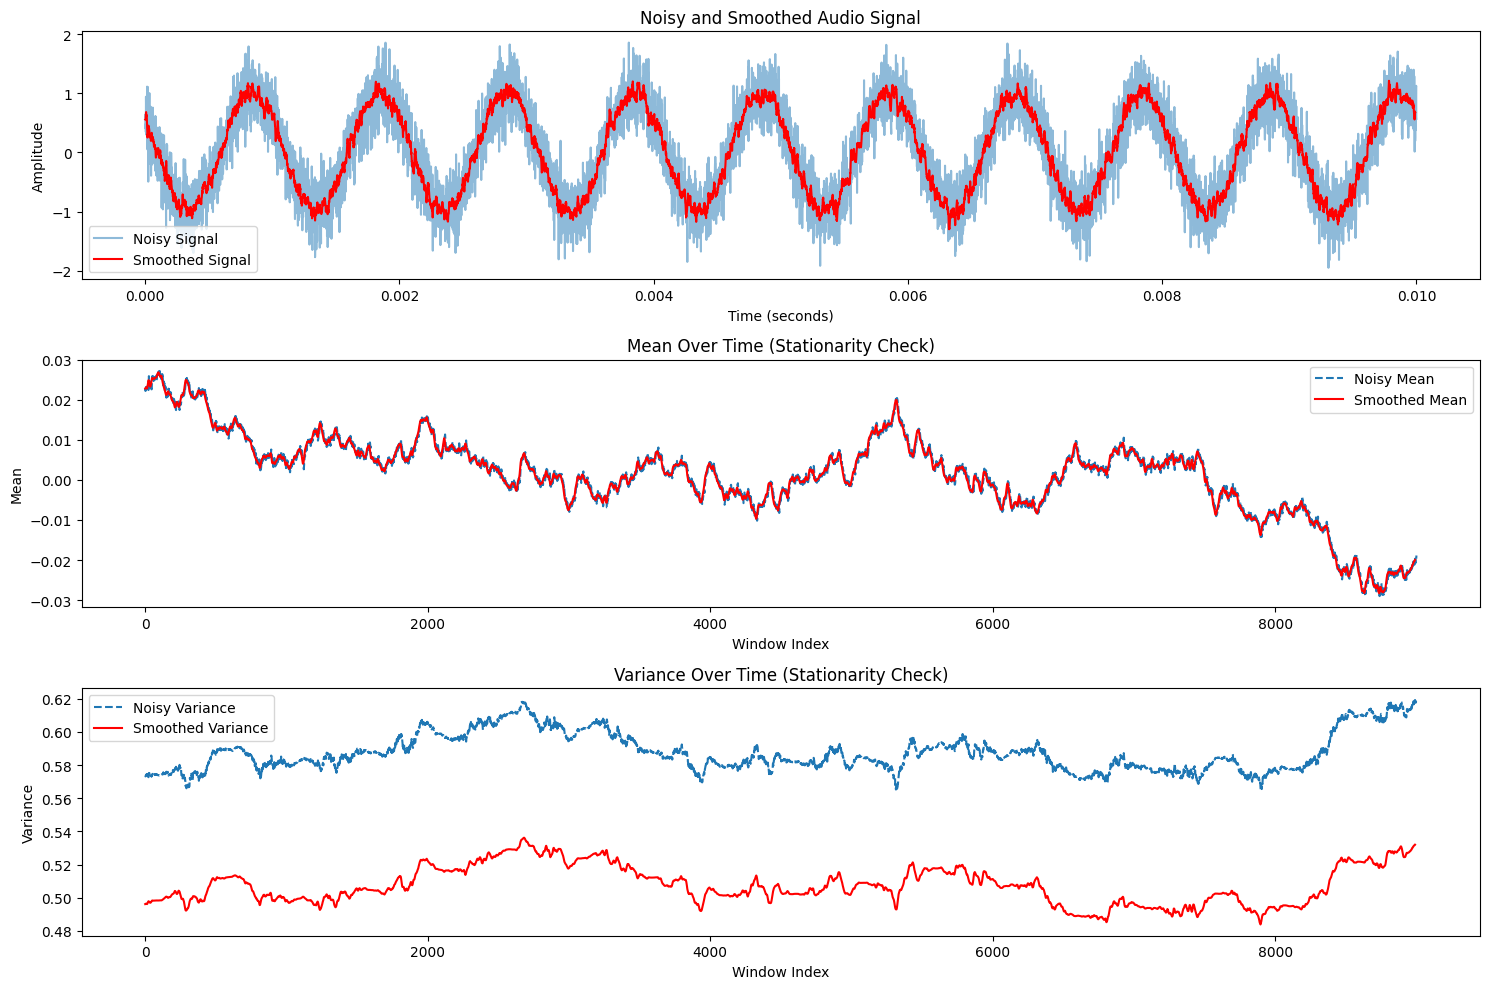
\includegraphics[width=0.8\textwidth]{Q3_GK_10.png}
\caption{Denoising with Gaussian Kernel}
\end{figure}

\clearpage
\subsubsection{ Denoising with Low Pass Butterworth Filter}
with a cutoff frequency of 0.1 and order of 5, the low pass butterworth filter denoising technique was applied to the data. The results are shown in figure 31.
\begin{figure}[h]
\centering
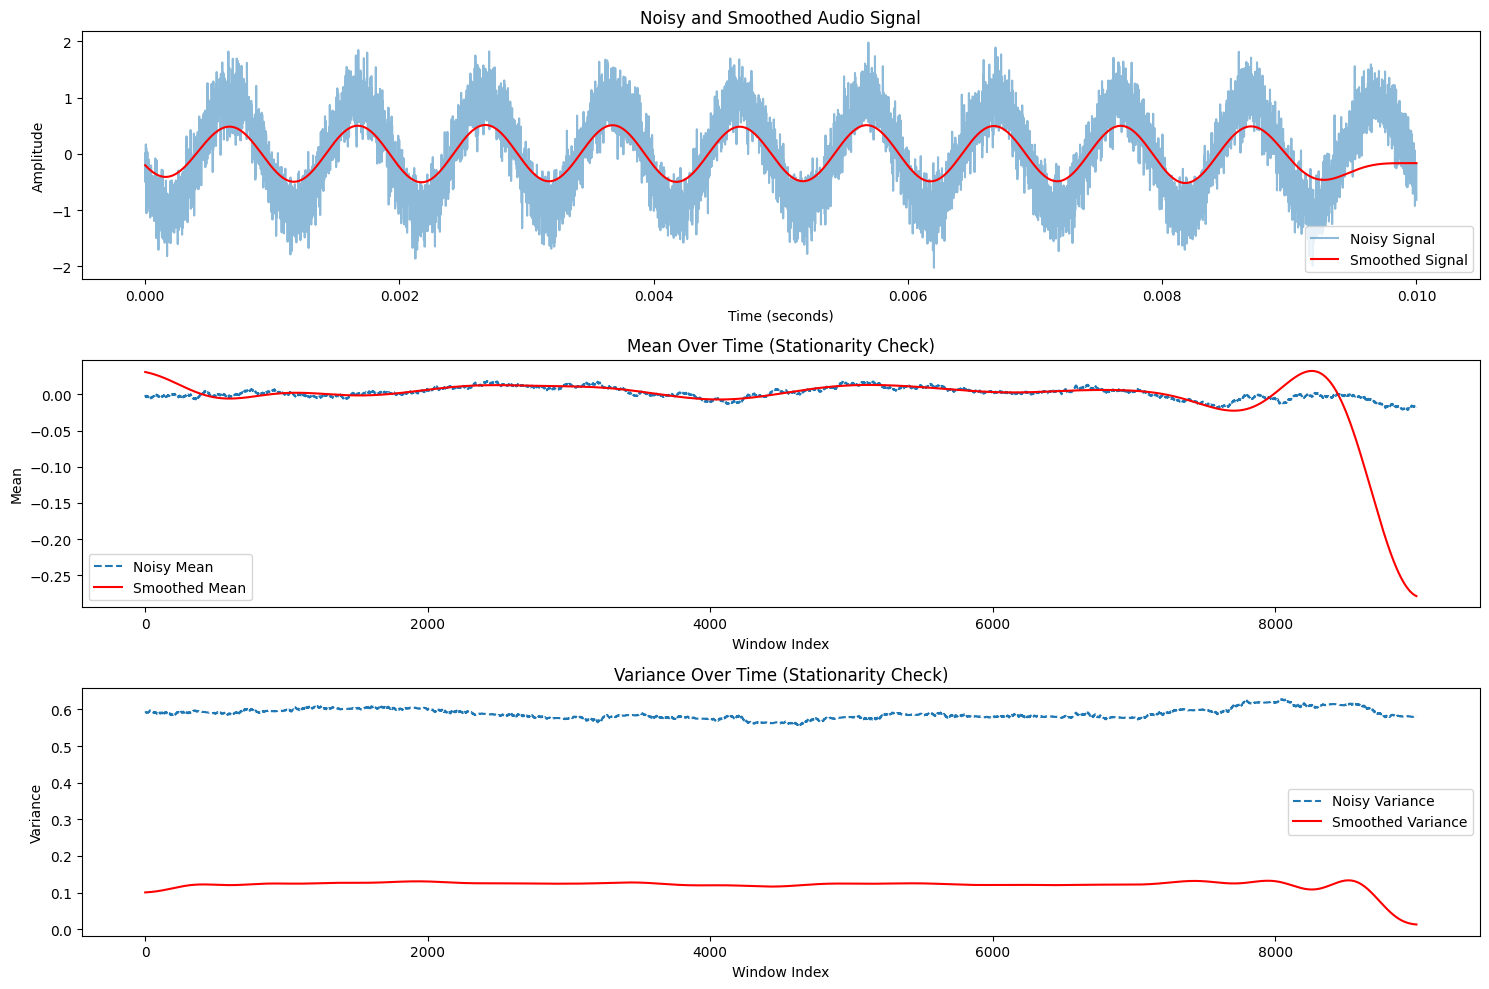
\includegraphics[width=0.8\textwidth]{Q3_LPB_0.1_1.png}
\caption{Denoising with Low Pass Butterworth Filter}
\end{figure}
\clearpage
with a cutoff frequency of 0.1 and order of 1, the low pass butterworth filter denoising technique was applied to the data. The results are shown in figure 32.
\begin{figure}[h]
\centering
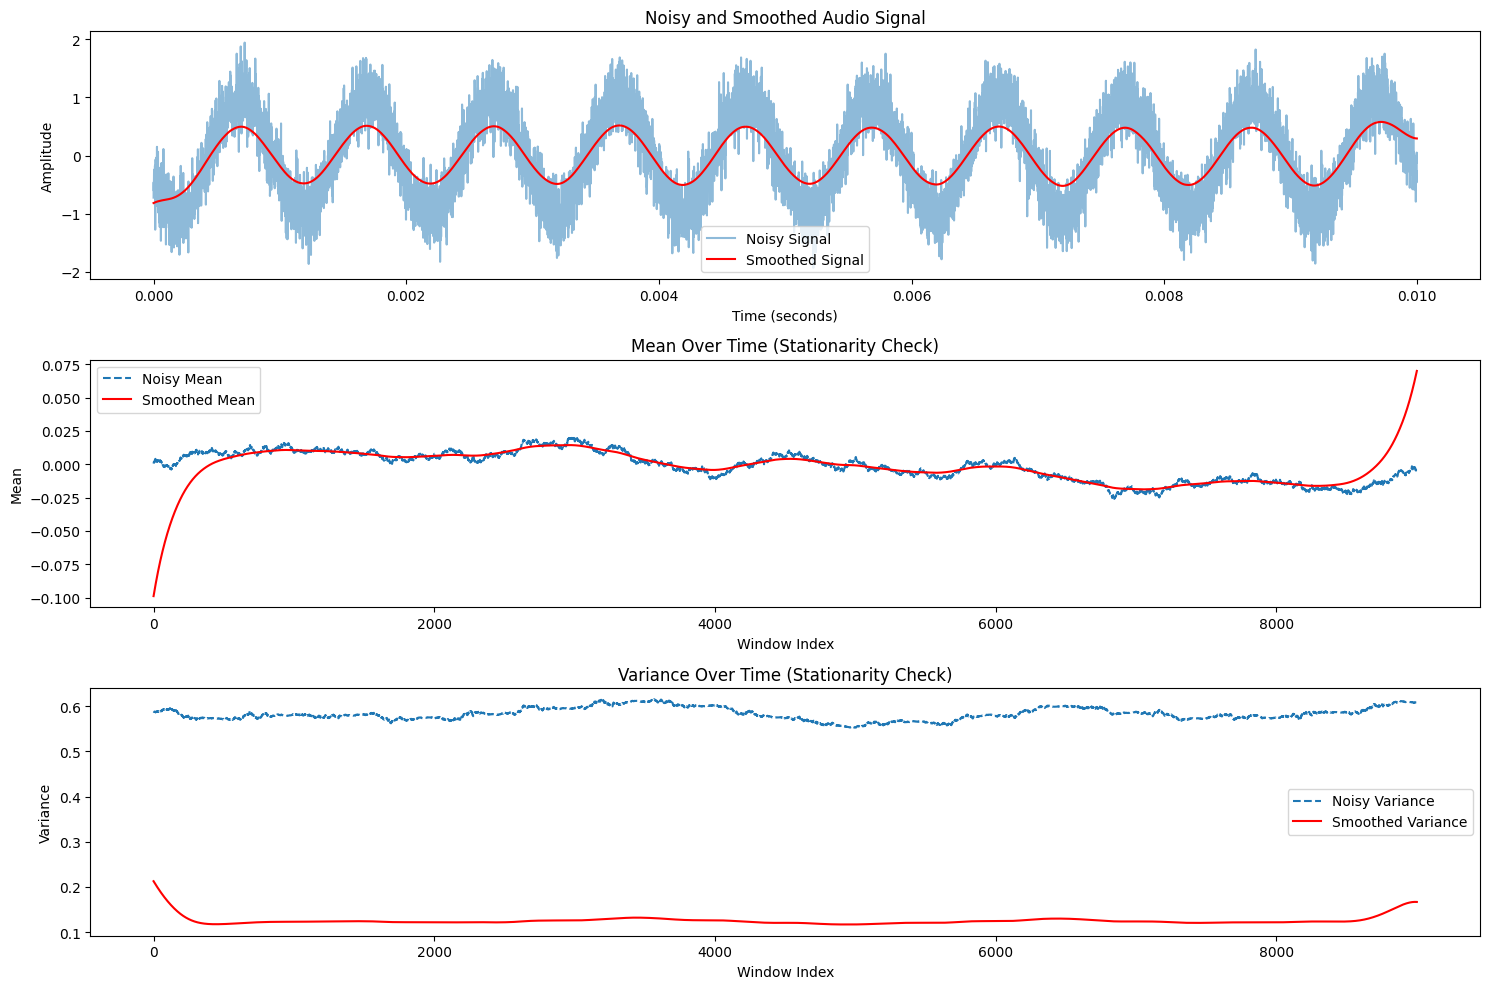
\includegraphics[width=0.8\textwidth]{Q3_LPB_0.1_2.png}
\caption{Denoising with Low Pass Butterworth Filter}
\end{figure}
\clearpage
with a cutoff frequency of 0.01 and order of 1, the low pass butterworth filter denoising technique was applied to the data. The results are shown in figure 33.
\begin{figure}[h]
\centering
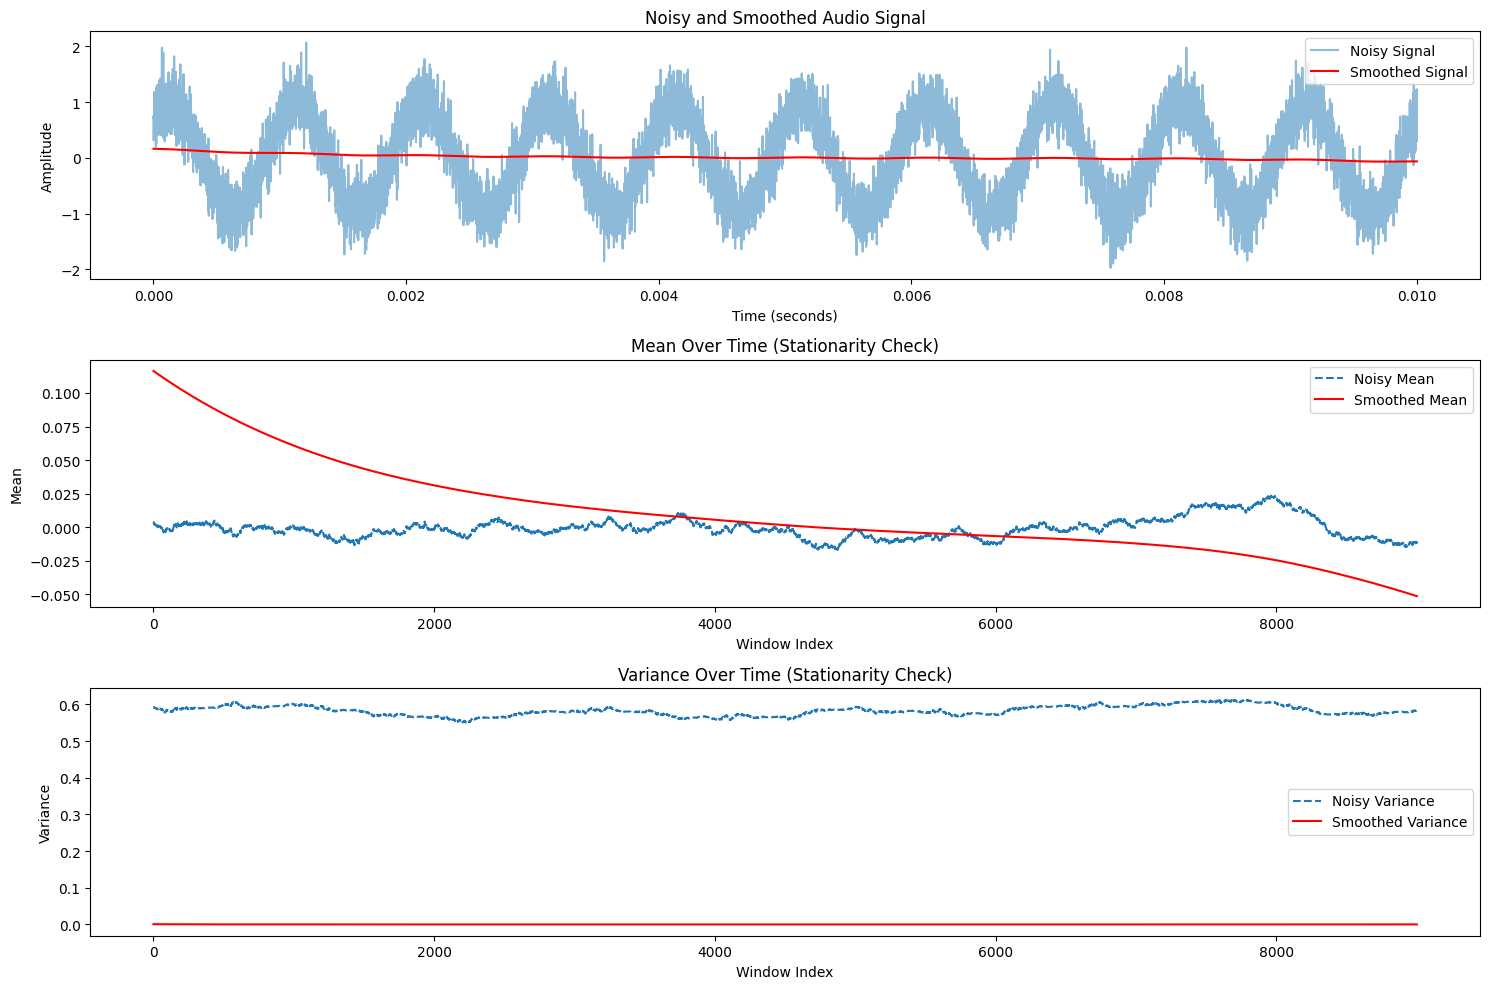
\includegraphics[width=0.8\textwidth]{Q3_LPB_0.01_1.png}
\caption{Denoising with Low Pass Butterworth Filter}
\end{figure}
\clearpage
with a cutoff frequency of 0.01 and order of 5, the low pass butterworth filter denoising technique was applied to the data. The results are shown in figure 34.
\begin{figure}[h]
\centering
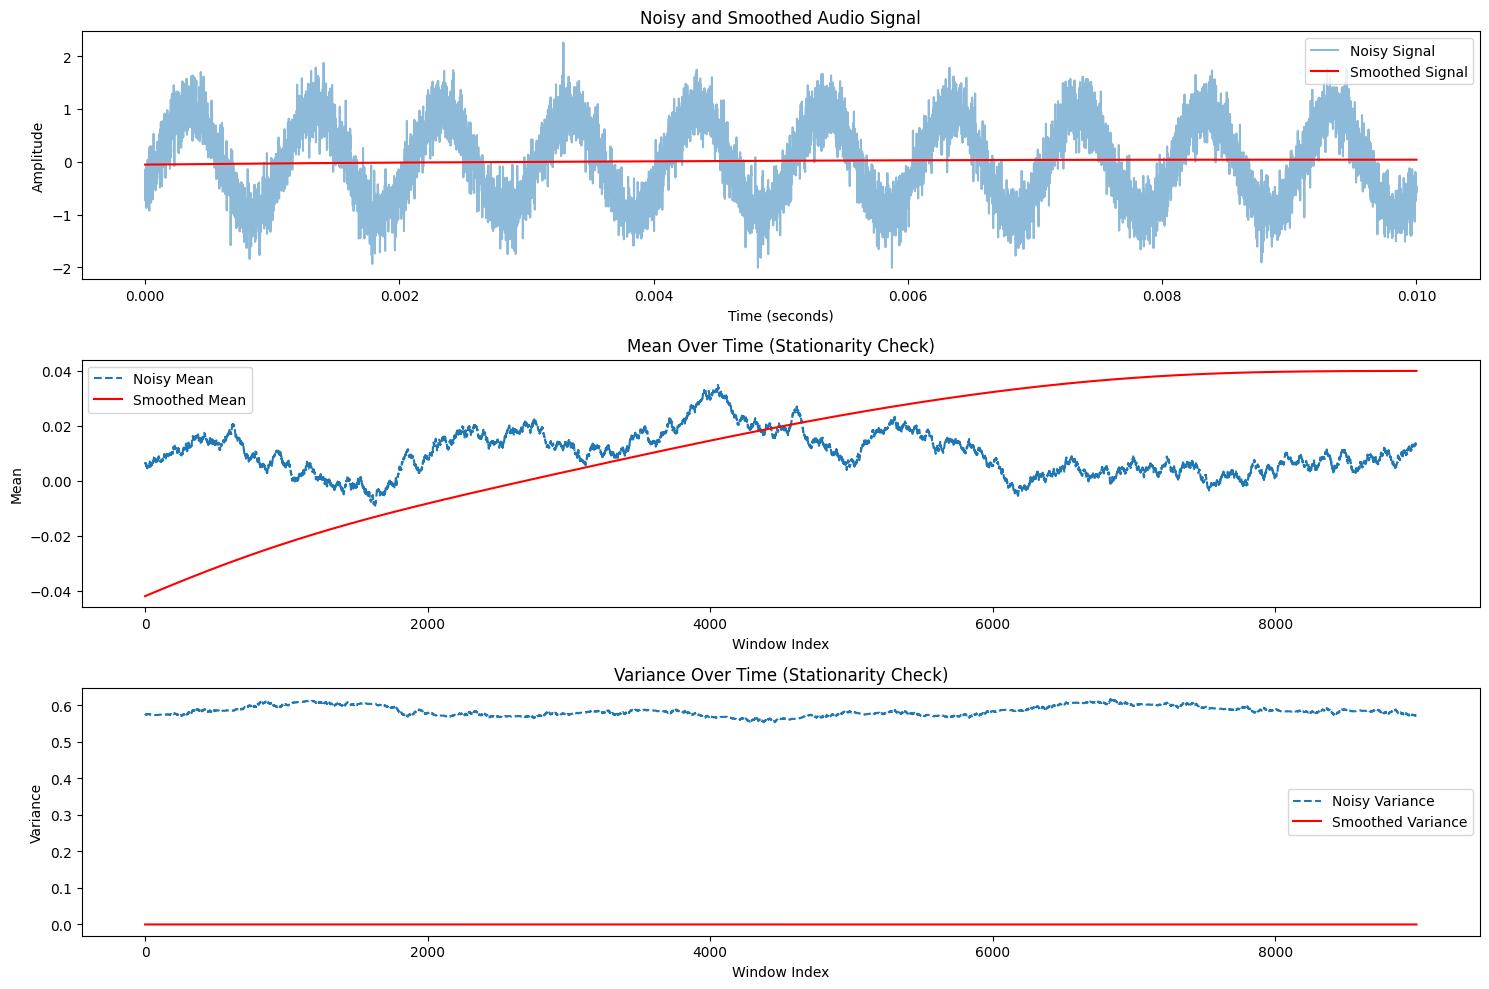
\includegraphics[width=0.8\textwidth]{Q3_LPB_0.01_5.png}
\caption{Denoising with Low Pass Butterworth Filter}
\end{figure}

\clearpage
\subsubsection{ Denoising with Exponential Moving Average}
with a smoothing parameter of 0.1, the exponential moving average denoising technique was applied to the data. The results are shown in figure 35.
\begin{figure}[h]
\centering
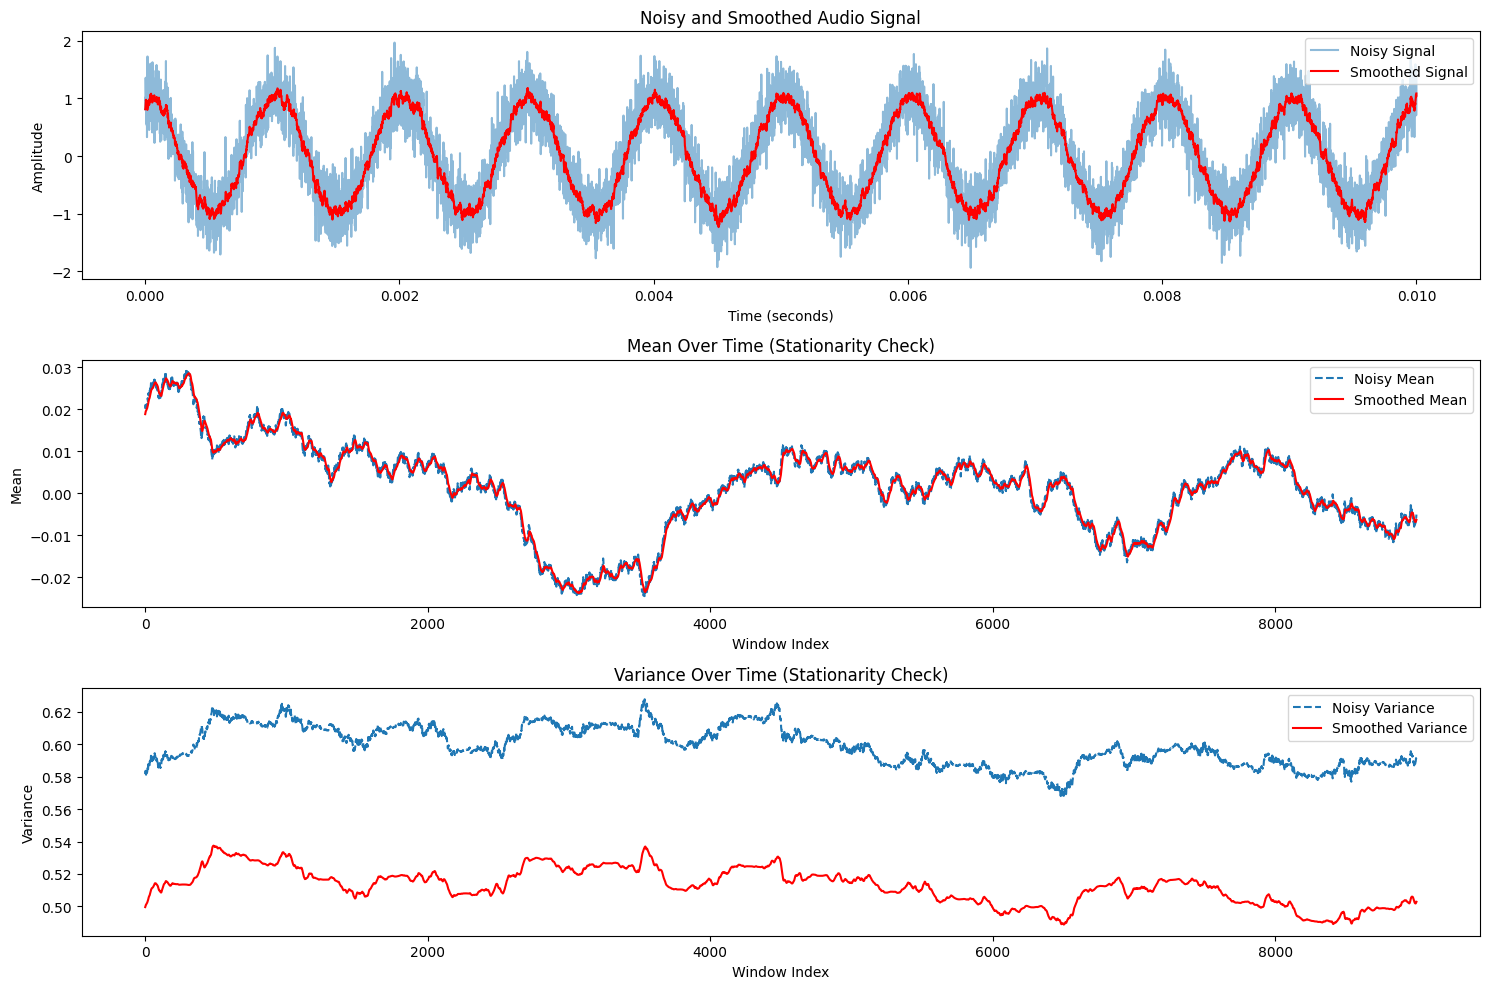
\includegraphics[width=0.8\textwidth]{Q3_EMA_0.1.png}
\caption{Denoising with Exponential Moving Average}
\end{figure}
\clearpage
with a smoothing parameter of 0.5, the exponential moving average denoising technique was applied to the data. The results are shown in figure 36.
\begin{figure}[h]
\centering
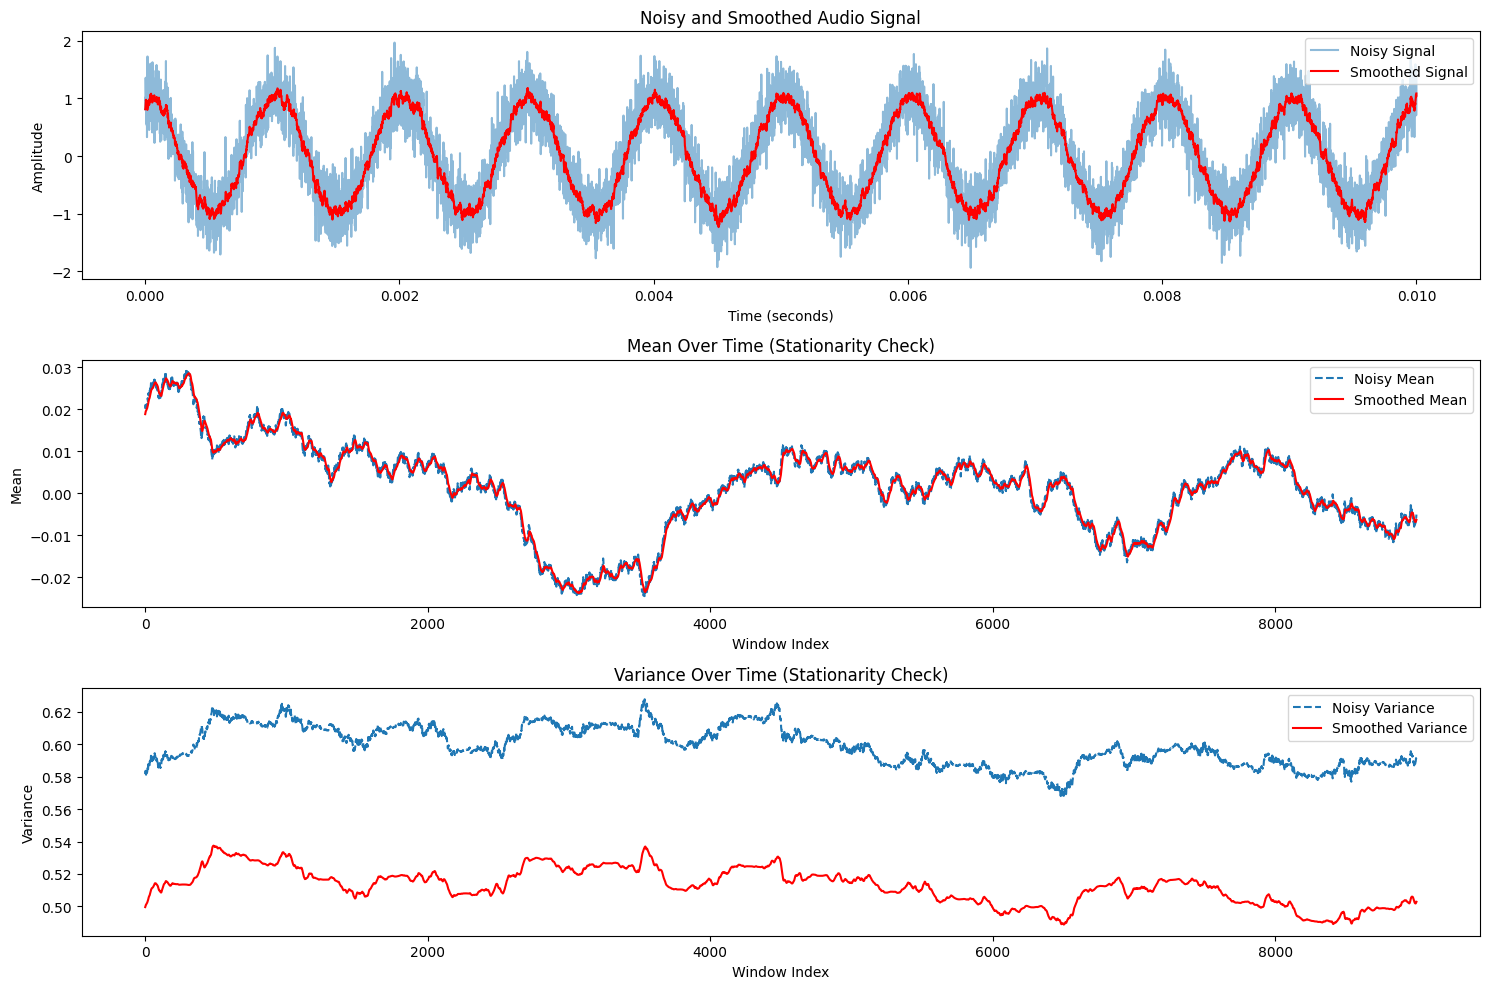
\includegraphics[width=0.8\textwidth]{Q3_EMA_0.5.png}
\caption{Denoising with Exponential Moving Average}
\end{figure}
\clearpage
with a smoothing parameter of 0.9, the exponential moving average denoising technique was applied to the data. The results are shown in figure 37.
\begin{figure}[h]
\centering
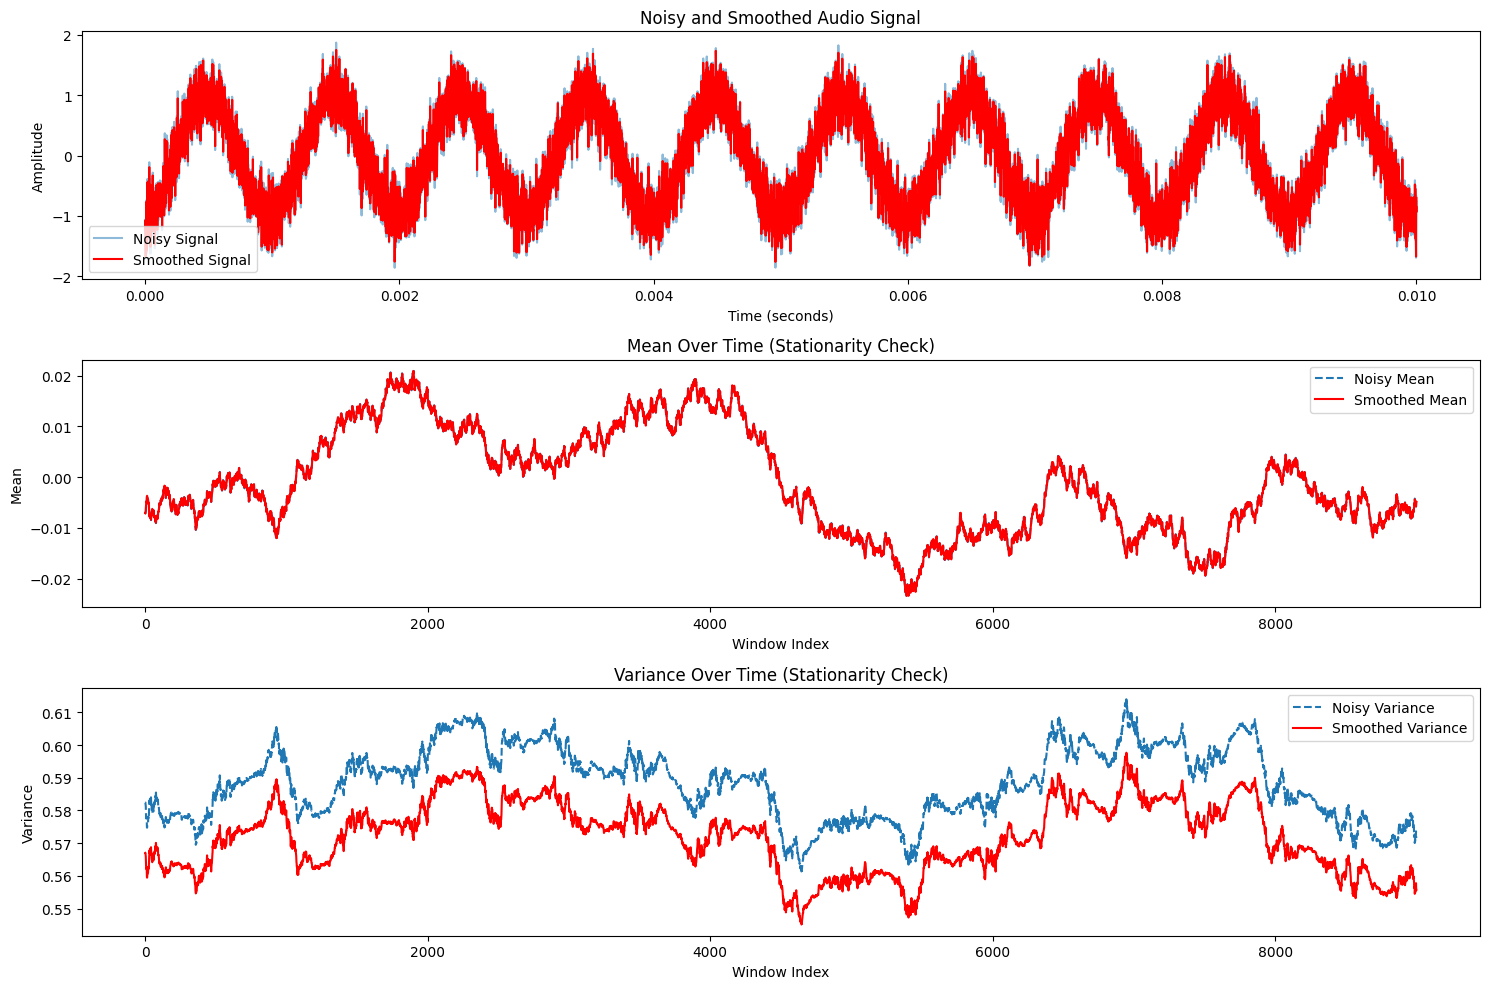
\includegraphics[width=0.8\textwidth]{Q3_EMA_0.9.png}
\caption{Denoising with Exponential Moving Average}
\end{figure}

\clearpage
\subsubsection{Reflection points}
\textbf{How does noise affect the stationarity of the audio signal (i.e., its mean and variance
over time)?}
Noise affects the stationarity of the audio signal by increasing the mean and variance over time. The mean and variance of the audio signal are higher when there is more noise in the data. This means that the audio signal is less stationary when there is more noise. The mean and variance of the audio signal are lower when there is less noise in the data. This means that the audio signal is more stationary when there is less noise. Overall, noise affects the stationarity of the audio signal by increasing the mean and variance over time.
\newline\newline
\textbf{How does smoothing restore stationarity? Which method is most effective?}
Smoothing restores stationarity by removing the noise from the data. This makes the mean and variance of the audio signal more stable over time. The audio signal becomes more stationary when the noise is removed. The Gaussian kernel and exponential moving average are the most effective methods for restoring stationarity. The Gaussian kernel assigns higher weights to more data points and the exponential moving average assigns higher weights to more recent data points. This makes these methods more accurate in recovering the original signal. The simple moving average and low pass butterworth filter did not work as well for this scenario. The denoised mean was further away from the true mean for these methods. This means that the simple moving average and low pass butterworth filter are not as accurate in recovering the original signal. Overall, I would recommend using the Gaussian kernel and exponential moving average for this scenario because they are more accurate in recovering the original signal.
\newline\newline
\textbf{Why is stationarity important in signal processing and time-series analysis?}
Stationarity is important in signal processing and time-series analysis because it helps identify underlying patterns in the data. Stationarity means that the mean and variance of the data are stable over time. This makes it easier to analyze the data and identify trends and patterns. For example, in time-series analysis, stationarity can help predict future trends and understand the underlying factors that influence the data. Stationarity is also important in signal processing because it helps remove noise from the data. This makes the data more reliable and accurate. Overall, stationarity is important in signal processing and time-series analysis because it helps identify underlying patterns in the data and make the data more reliable and accurate.
\newline\newline
\textbf{Explain the impact of smoothing on stationarity and discuss practical applications.}
Smoothing has a positive impact on stationarity by removing noise from the data. This makes the mean and variance of the data more stable over time. The data becomes more stationary when the noise is removed. This can help identify underlying patterns in the data and make the data more reliable and accurate. In practical applications, smoothing can be used to improve the quality of measurements in various fields such as medical testing, manufacturing quality control, and audio signal processing. For example, in medical testing, smoothing can help remove noise from the measurements and make the data more reliable. In manufacturing quality control, smoothing can help improve the accuracy of the measurements and identify underlying patterns in the data. In audio signal processing, smoothing can help remove noise from the audio signal and make the data more reliable and accurate. Overall, smoothing has a positive impact on stationarity and can be used to improve the quality of measurements in various fields.
\section{CONCLUSION}
This homework explored the use of various denoising techniques such as the simple moving average, Gaussian kernel, low pass Butterworth filter, and exponential moving average. 

\subsection*{Key Findings}
\begin{itemize}
    \item \textbf{Quality Control with Noisy Measurements:} The Gaussian kernel and exponential moving average were found to be the most effective denoising techniques. They provided denoised means closer to the true mean compared to the simple moving average and low pass Butterworth filter.
    \item \textbf{Temperature Trends with Noisy Measurements:} Smoothing improved the visibility of seasonal trends in the autocorrelation plot. The Gaussian kernel and exponential moving average were again the most effective methods for this scenario.
    \item \textbf{Stationarity Analysis of an Audio Signal:} Noise increased the mean and variance of the audio signal, making it less stationary. Smoothing restored stationarity, with the Gaussian kernel and exponential moving average being the most effective methods.
\end{itemize}

\subsection*{Broader Implications}
Noise and denoising have significant implications in real-world scenarios. In fields such as medical testing, manufacturing quality control, and audio signal processing, noise can obscure important patterns and trends. Effective denoising techniques can improve the accuracy and reliability of measurements, leading to better decision-making and outcomes.

\subsection*{Effectiveness of Denoising Techniques}
The Gaussian kernel and exponential moving average consistently outperformed the simple moving average and low pass Butterworth filter across different tasks. These methods provided more accurate recovery of the original signal by assigning appropriate weights to data points.

\subsection*{Recommendations}
\begin{itemize}
    \item \textbf{Gaussian Kernel:} Recommended for scenarios where it is important to assign weights to data points based on their distance from the center of the kernel. Suitable for applications in quality control and temperature trend analysis.
    \item \textbf{Exponential Moving Average:} Recommended for scenarios where recent data points should be given higher weights. Suitable for applications in financial data analysis and real-time signal processing.
    \item \textbf{Simple Moving Average and Low Pass Butterworth Filter:} These methods can be used for basic denoising tasks but may not be as effective in scenarios requiring high accuracy.
\end{itemize}

Overall, the choice of denoising method should be based on the specific requirements of the application and the nature of the data. The Gaussian kernel and exponential moving average are generally more effective for achieving accurate denoising results.

\end{document}